%%%%%%%%%%%%%%%%%%%%%%%%%%%%%%%%%%%%%%%%%%%%%%%%%%%%%%%%%%%%%%%%%%%%%%%
%
%  Honours Thesis
%  Smarak Nayak 
%  2016
%
%%%%%%%%%%%%%%%%%%%%%%%%%%%%%%%%%%%%%%%%%%%%%%%%%%%%%%%%%%%%%%%%%%%%%%%
%
%  The first part pulls in a UNSW Thesis class file.  This one is
%  slightly nonstandard and has been set up to do a couple of
%  things automatically
%
 
\documentclass[honours,12pt]{unswthesis}
\linespread{1.3}
\usepackage{amsfonts}
\usepackage{amssymb}
\usepackage{amsthm}
\usepackage{latexsym,amsmath}
\usepackage{graphicx}
\usepackage{afterpage}

%Peter's packages
\usepackage{color}
\usepackage{lineno} %for line numbers
\usepackage{enumerate}
\usepackage{url}
\usepackage{hyperref}
\usepackage{doi}

\usepackage{float}
\usepackage{bbm}
%%%%%%%%%%%%%%%%%%%%%%%%%%%%%%%%%%%%%%%%%%%%%%%%%%%%%%%%%%%%%%%%%
%
%  The following are some simple LaTeX macros to give some
%  commonly used letters in funny fonts. You may need more or less of
%  these
%
\newcommand{\R}{\mathbb{R}}
\newcommand{\Q}{\mathbb{Q}}
\newcommand{\C}{\mathbb{C}}
\newcommand{\N}{\mathbb{N}}
\newcommand{\F}{\mathbb{F}}
\newcommand{\PP}{\mathbb{P}}
\newcommand{\T}{\mathbb{T}}
\newcommand{\Z}{\mathbb{Z}}
\newcommand{\B}{\mathfrak{B}}
\newcommand{\BB}{\mathcal{B}}
\newcommand{\M}{\mathfrak{M}}
\newcommand{\X}{\mathfrak{X}}
\newcommand{\Y}{\mathfrak{Y}}
\newcommand{\CC}{\mathcal{C}}
\newcommand{\E}{\mathbb{E}}
\newcommand{\cP}{\mathcal{P}}
\newcommand{\cS}{\mathcal{S}}
\newcommand{\A}{\mathcal{A}}
\newcommand{\ZZ}{\mathcal{Z}}

%Peter's commands
\newcommand{\ex}{\mathbf {E}}
\newcommand{\pr}{\mathbf {P}}
\newcommand{\Rd}{\mathbb R^d}
\newcommand{\Rp}{\mathbb R^+}
\newcommand{\spctim}{\mathbb R^{d+1}}
\newcommand{\del}{\partial }
\newcommand{\1}{\mathbf 1}
\newcommand{\eps}{\varepsilon}

%Other commands
\newcommand{\FF}{\mathcal{F}}
\newcommand{\Law}{\mathop{\rm Law}}
\newcommand{\Cov}{\mathop{\rm Cov}}
\newcommand{\Var}{\mathop{\rm Var}}
\newcommand{\sign}{\mathop{\rm sign}}
\newcommand{\Floor}[1]{{\lfloor {#1} \rfloor}}
\newcommand{\cd}{\overset{d}{\longrightarrow}}
\newcommand{\D}{\mathbb{D}}
\newcommand{\ppartial}[2]{\dfrac{\partial {#1}}{\partial {#2} }}


%%%%%%%%%%%%%%%%%%%%%%%%%%%%%%%%%%%%%%%%%%%%%%%%%%%%%%%%%%%%%%%%%%%%%
%
% The following are much more esoteric commands that I have left in
% so that this file still processes. Use or delete as you see fit
%
\newcommand{\bv}[1]{\mbox{BV($#1$)}}
\newcommand{\comb}[2]{\left(\!\!\!\begin{array}{c}#1\\#2\end{array}\!\!\!\right)
}
\newcommand{\Lat}{{\rm Lat}}
\newcommand{\var}{\mathop{\rm var}}
\newcommand{\Pt}{{\mathcal P}}
\def\tr(#1){{\rm trace}(#1)}
\def\Exp(#1){{\mathbb E}(#1)}
\def\Exps(#1){{\mathbb E}\sparen(#1)}
\newcommand{\floor}[1]{\left\lfloor #1 \right\rfloor}
\newcommand{\ceil}[1]{\left\lceil #1 \right\rceil}
\newcommand{\hatt}[1]{\widehat #1}
\newcommand{\modeq}[3]{#1 \equiv #2 \,(\text{mod}\, #3)}
\newcommand{\rmod}{\,\mathrm{mod}\,}
\newcommand{\p}{\hphantom{+}}
\newcommand{\vect}[1]{\mbox{\boldmath $ #1 $}}
\newcommand{\reff}[2]{\ref{#1}.\ref{#2}}
\newcommand{\psum}[2]{\sum_{#1}^{#2}\!\!\!'\,\,}
\newcommand{\bin}[2]{\left( \begin{array}{@{}c@{}}
				#1 \\ #2
			\end{array}\right)	}
%
%  Macros - some of these are in plain TeX (gasp!)
%
\newcommand{\be}{($\beta$)}
\newcommand{\eqp}{\mathrel{{=}_p}}
\newcommand{\ltp}{\mathrel{{\prec}_p}}
\newcommand{\lep}{\mathrel{{\preceq}_p}}
\def\brack#1{\left \{ #1 \right \}}
\def\bul{$\bullet$\ }
\def\cl{{\rm cl}}
\let\del=\partial
\def\enditem{\par\smallskip\noindent}
\def\implies{\Rightarrow}
\def\inpr#1,#2{\t \hbox{\langle #1 , #2 \rangle} \t}
\def\ip<#1,#2>{\langle #1,#2 \rangle}
\def\lp{\ell^p}
\def\maxb#1{\max \brack{#1}}
\def\minb#1{\min \brack{#1}}
\def\mod#1{\left \vert #1 \right \vert}
\def\norm#1{\left \Vert #1 \right \Vert}
\def\paren(#1){\left( #1 \right)}
\def\qed{\hfill \hbox{$\Box$} \smallskip}
\def\sbrack#1{\Bigl \{ #1 \Bigr \} }
\def\ssbrack#1{ \{ #1 \} }
\def\smod#1{\Bigl \vert #1 \Bigr \vert}
\def\smmod#1{\bigl \vert #1 \bigr \vert}
\def\ssmod#1{\vert #1 \vert}
\def\sspmod#1{\vert\, #1 \, \vert}
\def\snorm#1{\Bigl \Vert #1 \Bigr \Vert}
\def\ssnorm#1{\Vert #1 \Vert}
\def\sparen(#1){\Bigl ( #1 \Bigr )}

\newcommand\blankpage{%
    \null
    \thispagestyle{empty}%
    \addtocounter{page}{-1}%
    \newpage}

%%%%%%%%%%%%%%%%%%%%%%%%%%%%%%%%%%%%%%%%%%%%%%%%%%%%%%%%%%%%%%
%
% These environments allow you to get nice numbered headings
%  for your Theorems, Definitions etc.  
%
%  Environments
%
%%%%%%%%%%%%%%%%%%%%%%%%%%%%%%%

\newtheorem{theorem}[equation]{Theorem}
\newtheorem{lemma}[equation]{Lemma}
\newtheorem{proposition}[equation]{Proposition}
\newtheorem{corollary}[equation]{Corollary}
\newtheorem{definition}[equation]{Definition}
\newtheorem{example}[equation]{Example}
\newtheorem{remark}[equation]{Remark}
\newtheorem{question}[equation]{Question}
\newtheorem{notation}[equation]{Notation}
\numberwithin{equation}{section}

%Peter's Environments
\newtheorem{cor}[equation]{Corollary}
\theoremstyle{definition}
\newtheorem{defi}[equation]{Definition}
\theoremstyle{remark}
%\newtheorem{remark}[equation]{Remark}

%%%%%%%%%%%%%%%%%%%%%%%%%%%%%%%%%%%%%%%%%%%%%%%%%%%%%%%%%%%%%%%%%%
%
%  If you've got some funny special words that LaTeX might not
% hyphenate properly, you can give it a helping hand:
%
\hyphenation{Mar-cin-kie-wicz Rade-macher}

%%%%%%%%%%%%%%%%%%%%%%%%%%%%%%%%%%%%%%%%%%%%%%%%%%%%%%%%%%%%%%%%%%
% 
% OK...Now we get to some actual input.  The first part sets up
% the title etc that will appear on the front page
%
%%%%%%%%%%%%%%%%%%%%%%%%%%%%%%%%%%%%%%%%%%%%%%%%%%%%%%%%%%%%%%%%%

\title{Statistics of Bursty Events}

\authornameonly{Smarak Nayak}

\author{\Authornameonly\\{\bigskip}Supervisor: Dr. Peter Straka}

\copyrightfalse
\figurespagefalse
\tablespagefalse

%%%%%%%%%%%%%%%%%%%%%%%%%%%%%%%%%%%%%%%%%%%%%%%%%%%%%%%%%%%%%%%%%
%
%  And now the document begins
%  The \beforepreface and \afterpreface commands puts the
%  contents page etc in
%
%%%%%%%%%%%%%%%%%%%%%%%%%%%%%%%%%%%%%%%%%%%%%%%%%%%%%%%%%%%%%%%%%%

\begin{document}

\beforepreface

\afterpage{\blankpage}

% plagiarism

\prefacesection{Plagiarism statement}

\vskip 10pc \noindent I declare that this thesis is my
own work, except where acknowledged, and has not been submitted for
academic credit elsewhere. 

\vskip 2pc  \noindent I acknowledge that the assessor of this
thesis may, for the purpose of assessing it:
\begin{itemize}
\item Reproduce it and provide a copy to another member of the University; and/or,
\item Communicate a copy of it to a plagiarism checking service (which may then retain a copy of it on its database for the purpose of future plagiarism checking).
\end{itemize}

\vskip 2pc \noindent I certify that I have read and understood the University Rules in
respect of Student Academic Misconduct, and am aware of any potential plagiarism penalties which may 
apply.\vspace{24pt}

\vskip 2pc \noindent By signing 
this declaration I am
agreeing to the statements and conditions above.
\vskip 2pc \noindent
Signed: \rule{7cm}{0.25pt} \hfill Date: \rule{4cm}{0.25pt} \newline
\vskip 1pc

\afterpage{\blankpage}

% Acknowledgements are optional


\prefacesection{Acknowledgements}

{\bigskip}By far the greatest thanks must go to my supervisor for
the guidance, care and support they provided. 

{\bigskip\noindent}Thanks 
must also go to Emily, Michelle, John and Alex who helped by
proof-reading the document in the final stages of preparation.

{\bigskip\noindent}Although
I have not lived with them for a number of years, my family also deserve
many thanks for their encouragement.

{\bigskip\noindent} Thanks go to Robert Taggart for allowing his thesis
style to be shamelessly copied.

{\bigskip\bigskip\bigskip\noindent} Fred Flintstone, 2 November 2015.

\afterpage{\blankpage}

% Abstract

\prefacesection{Abstract}

The prediction of extreme events resulting from human
behaviour is becoming significant in areas as far reaching as the
control of disease spread, resource allocation, and emergency
response.  Classical methods in extreme value theory fail to recognise
that most human created events do not occur uniformly, but in bursts.
In this thesis, 
extremes of bursty events are modelled via Continuous Time Random Maxima
(CTRM) with heavy-tailed waiting times.  Methods for Statistical Inference
are developed. 
\afterpage{\blankpage}


\afterpreface

%%%%%%%%%%%%%%%%%%%%%%%%%%%%%%%%%%%%%%%%%%%%%%%%%%%%%%%%%%%%%%%%%%
%
% Now we can start on the first chapter
% Within chapters we have sections, subsections and so forth
%
%%%%%%%%%%%%%%%%%%%%%%%%%%%%%%%%%%%%%%%%%%%%%%%%%%%%%%%%%%%%%%%%%%

\afterpage{\blankpage}

\chapter{Introduction}\label{s-intro}
Time series displaying inhomogeneous behaviour have received strong interest in 
the recent statistical physics literature,
\cite{Barabasi2005,Oliveira2005,Vasquez2006,Vazquez2007,Omi2011,
Min2010,Karsai2011,Bagrow2013},
and have been observed in the context of earthquakes, sunspots, neuronal
activity, human communication etc., see \cite{Karsai2012,Vajna2013} for a 
list of references.
Such time series exhibit high activity in some `bursty' intervals, which 
alternate with other, quiet intervals.  Although several mechanisms are 
plausible explanations for bursty behaviour
(most prominently self-exciting point processes \cite{hawkes1971point}),
there seems to be one salient
feature which very typically indicates the departure from temporal homogeneity: 
A heavy-tailed distribution of waiting times
\cite{Vasquez2006,Karsai2012,Vajna2013}. 
A simple renewal process with heavy-tailed waiting times captures these
dynamics. For many systems, the renewal property is appropriate, as can be
checked by a simple test: the dynamics do not change visibly if the
waiting times are randomly reshuffled \cite{Karsai2012}.

When a magnitude can be assigned to each event in the renewal process, 
such as for earthquakes, sun flares, neuron voltages or the impact of an email,
two natural and basic questions to ask are: 
What is the distribution of the largest event up to a given time $t$?
What is the probability that an event exceeds a given level $\ell$ within the
next $t$ units of time?
A probabilistic extreme value model which assumes that the events form a 
renewal process is available in the literature. 
This model has been studied under the names
``Continuous Time Random Maxima process'' (CTRM) 
\cite{Benson2007,Meerschaert2009,Hees16,Hees2015}, 
``Max-Renewal process'' \cite{Silvestrov2002a,ST04,Basrak2014}, 
and ``Shock process'' 
\cite{Esary1973,Sumita1983,Sumita1984,Sumita1985,Anderson1987,Gut1999}.
This thesis aims to develop concrete statistical inference methods for this model, 
a problem which has seemingly received little attention by the statistical 
community.

\chapter{Preliminaries}\label{prelim}
In this chapter, we introduce the notation and review the background theory of probability and stochastic processes that are necessary in developing the statistical methods outlined in this thesis.
\section{Probability and Measure Theory}

\begin{definition}
Let $\Omega$ be a nonempty set and let $\FF$ be a collection of subsets of $\Omega$. We say that $\FF$ is a \textbf{$\sigma$-algebra} if it satisfies the following conditions
\begin{enumerate}
\item The empty set $\emptyset \in \FF$,
\item If $A\in \FF$ then the complement $A^c\in \FF$, and
\item If $A_1,A_2,\ldots \in \FF$ then their union $\bigcup_{n=1}^\infty A_n \in \FF$.
\end{enumerate}
\end{definition}
\noindent It follows that a $\sigma$-algebra is also closed under intersection.\\
\begin{definition}
Let $\Omega$ be a nonempty set and let $\FF$ be a $\sigma$-algebra on $\Omega$. Then the pair $(\Omega,\FF)$ is called a \textbf{measurable space}.\\
\end{definition}

\begin{definition}
Let $(\Omega,\FF)$ be a measurable space. A \textbf{measure} $\mu$ is a real-valued set function on $\FF$ satisfying the following conditions
\begin{enumerate}
\item For every set $A\in \FF$, $\mu(A) \geq 0$, and
\item If $A_1, A_2,\ldots$ is a sequence of disjoint sets in $\FF$ then 
\[
\mu\left(\bigcup_{n=1}^\infty A_n\right) = \sum_{n=1}^\infty \mu(A_n).
\]
\end{enumerate}
\end{definition}
\noindent Now that the concept of a measure has been defined we can interpret a $\sigma$-algebra as the set of all events that can be measured from the underlying set $\Omega$.\\
\begin{definition}
Let $(\Omega,\FF)$ be a measurable space. A \textbf{probability measure} $\PP$ is a measure such that $\PP(\Omega) = 1$.\\
\end{definition}
\begin{definition}
Let $\mu$ be a measure defined on the measurable space $(\Omega,\FF)$. We call the triplet $(\Omega,\FF,\mu)$ a \textbf{measure space}. In particular, if $\PP$ is a probability measure then we call $(\Omega,\FF,\PP)$ a \textbf{probability space}.\\
\end{definition}

{\noindent}A particular example of a probability measure that we will use later on is the Dirac measure.\\
\begin{definition} Let $(\Omega, \FF)$ be some measurable space. A \textbf{Dirac measure} $\delta_x$ is a measure defined on a given point $x\in \Omega$ and a set $A\in \FF$ 
\[
\delta_x(A) = 
\begin{cases}
0, &x\notin A;\\
1, &x\in A.
\end{cases}
\]
\end{definition}
{\noindent}A useful result of Dirac measures is the identity
\[
\int f(y)\delta_x(dy) = f(x).
\]
The Dirac measure extends the concept of indicator functions to sets. Another example of a measure is the Lebesgue measure, which is the standard measure on the Euclidean space $\R^d$. The rigorous definition of a Lebesgue measure is fairly analytical and is omitted. The Lebesgue measure is essentially an extension of the standard notions of length, area and volume to $d$-dimensional Euclidean spaces.\\


\begin{definition}
Let $(\Omega,\FF)$ and $(E,\mathcal{E})$ be measurable spaces. Then a function $f: \Omega \rightarrow E$ is ($\FF,\mathcal{E}$)-\textbf{measurable} if $f^{-1}(S)\in \FF$ for every $S\in \mathcal{E}$.\\
\end{definition}

\begin{definition}
Let $(\Omega,\FF,\PP)$ be a probability space and $(E,\mathcal{E})$ a measurable space. A \textbf{random variable} is a function $X:\Omega \rightarrow E$ that is $(\FF,\mathcal{E})$-measurable. We call $(E,\mathcal{E})$ the \textbf{state space}. \\
\end{definition}

\begin{definition}
	Let X be a random variable defined on a probability space $(\Omega,\FF,\PP)$. Its \textbf{characteristic function} $\phi_X(s):\Omega\to\C$ is defined by 
	\begin{align*}
		\phi_X(s)&=\E[e^{isX}]\\
		&=\int_\Omega e^{isX(\omega)} \PP(d\omega)
	\end{align*}
	for every $s \in \R$.
\end{definition}

\section{Stochastic Processes}
Generally speaking, a stochastic process $\{X_t\}_{t\geq 0}$ is a collection of random variables that represent the evolution of some object over time. As this thesis focuses heavily on stochastic processes it is important that we rigorously define what a stochastic process is.\\

\begin{definition}
A \textbf{stochastic process} is a collection of random variables $\{X_t\}_{t\in \mathcal{I}}$ that is defined on a probability space $(\Omega, \FF,\PP)$ and is indexed by an ordered set $\mathcal{I}$. \\
\end{definition}

\noindent If we fix a $t_0\in \mathcal{I}$ then $X(t_0,\omega)$ is simply a random variable. If we fix a $\omega_0\in \Omega$ then $X(t,\omega_0)$ is a function with respect to $t$ and is the trajectory of a single realisation of the stochastic process $X(t)$. From now on we will only consider stochastic processes where our ordered set $\mathcal{I}=\Rp$ represents an interval in continuous time. We now write $\{X(t)\}_{t\geq 0}:\Rp\times\Omega\to\R$.\\ 

\begin{definition}
A stochastic process $\{X(t)\}_{t\geq 0}$ has a \textbf{jump} at time t if the process is discontinuous at that point. More precisely $X(t) \neq X_-(t)$.\\
\end{definition}

\begin{definition}
A stochastic process $\{X(t)\}_{t\geq 0}$ is \textbf{c\`{a}dl\`{a}g} (derived from the French term "continue \`{a} droite, limite \`{a} gauche") if it is continuous from the right
\[
	\lim_{\epsilon\to0+}X(t+\epsilon)=X(t),
\]
with left hand limits
\[
	\lim_{\epsilon\to0+}X(t-\epsilon)=X(t-).
\]
\end{definition}

\begin{definition}
A \textbf{filtration} $\{\FF_t\}_{t\geq 0}$ is a collection of $\sigma$-algebras such that for any $0\leq s \leq t$, $\FF_s \subseteq \FF_t$.\\
\end{definition}

{\noindent}Note that with each successive $\sigma$-algebra the amount of sets that can be measured is non-decreasing. Thus a filtration can be interpreted as the accumulation of information about our stochastic process with respect to time. We write $\sigma(X_s,s\leq t)$ as the smallest $\sigma$-algebra generated by $\{X_s: s\leq t\}$.\\

\begin{definition}
Let $(\Omega,\FF,\PP)$ be a probability space with the filtration $\FF = \{\FF\}_{t\geq 0}$ and let $(E,\mathcal{E})$ a measurable space. We say the stochastic process $\{X_t\}_{t\geq 0}$ is $\boldsymbol{\FF}$\textbf{- adapted} if for every $t\geq 0$, $X_t: \Omega \rightarrow E$ is $(\FF_t, \mathcal{E})$ - measurable.\\
\end{definition}

\begin{definition}
Let $(\Omega, \FF,\PP)$ be a probability space. A real valued stochastic process $\{W_t\}_{t\geq 0}$ with continuous paths is a \textbf{standard Brownian motion} if for all $0<s<t$,
\begin{itemize}
\item $W_0 = 0\ a.s.$,
\item $W_t - W_s \sim N(0,t-s)$, and
\item the increments $W_t - W_s$ are independent. That is, $W_t - W_s$ is independent of $\sigma(W_r,r\leq s)$.\\
\end{itemize}
\end{definition}

\section{Weak Convergence}
The notion of weak convergence or convergence in distribution is also required to understand results utilised in this thesis.\\

\begin{definition}
A \textbf{metric} $d$ on a set $E$ is a non-negative real-valued function on the product space $E\times E$ such that
	\begin{itemize}
		\item $d(x,y)=0$ iff $x=y,$
		\item $d(x,y)=d(y,x),$
		\item $d(x,z) \leq d(x,y)+d(y,z).$
	\end{itemize}
\end{definition}
\noindent A metric is a function that defines the distance between two points in a set.\\

\begin{definition}
Let E be a set and let d be a metric on E. Then the ordered pair (E,d) is a \textbf{metric space}.\\
\end{definition}

\begin{definition}\label{def:metricConvergence}
A sequence $\{x_n\}_{n\geq1}$ in a metric space (E,d) \textbf{converges to a limit} $x\in E$ if, for all $\epsilon>0$, there exists an integer $n_0$ such that $d(x_n,x)<\epsilon$ for all $n\geq n_0$.\\
\end{definition}

\begin{definition}
A sequence of probability measures $\{\PP_n\}_{n \geq 1}$ on the measurable space $(\Omega, \FF)$ \textbf{converges weakly} to a probability measure $\PP$ on $(\Omega, \FF)$ if
\[
\lim_{n\rightarrow \infty} \int_\Omega fd\PP_n = \int_\Omega fd\PP
\]
for all continuous and bounded real-valued functions $f$ on $\Omega$. We then write \[\PP_n\rightarrow\PP.\]
\end{definition}
\noindent Note that this definition is just \ref{def:metricConvergence} with $E$ as the set of all probability measures on the measurable space $(\Omega, \FF)$ and $d(\PP,\mathbb{Q})=|\int_\Omega fd\PP- \int_\Omega fd\mathbb{Q}|$, where $\mathbb{Q}$ is another probability measure on $(\Omega, \FF).$\\

\begin{definition}
Let $X_n:\Omega\to E$ be a sequence of random variables with a corresponding sequence of probability measures $\{\PP_{X_n}\}_{n\geq 1}$ on the measurable space $(\Omega, \FF)$. Then $\{X_n\}_{n\geq 1}$ \textbf{converges in distribution} to a random variable $X:\Omega\to E$ if 
\[
\PP_{X_n} \to \PP_X
\] where $\PP_X$ is the probability measure of X. We then write $X_n \overset{d}{\to}X.$\\
\end{definition}

\begin{definition}\label{def:equalDist}
Let $X_1:\Omega\to E$ be a  random variable with a corresponding probability measure $\PP_{X_1}$ on the measurable space $(\Omega, \FF)$. Then $X_1$ is \textbf{equal in distribution} to a random variable $X_2:\Omega\to E$ if 
\[\PP_{X_1} = \PP_{X_2} \] where $\PP_{X_2}$ is the probability measure of $X_2$. We then write $X_1 \overset{d}{=}X_2$ or $X_1 \sim X_2$.\\
\end{definition}

\section{The Skorokhod Space}
The stochastic processes we will be discussing in this thesis will not necessarily be continuous as they may contain jumps. Thus it is necessary to consider the Skorokhod space, which is the space of such processes, and its associated theory in order to examine the convergence of stochastic processes with jumps.\\
\begin{definition}
	The \textbf{Skorokhod Space} $\D(\mathcal{I},\R^d)$ is the set of all $\R^d$-valued c\`{a}dl\`{a}g functions defined on a subinterval $\mathcal{I}$ of the real line.\\
\end{definition}

\noindent In order to properly discuss convergence in Skorokhod space we will assign it a metric. Let us first consider the simplest case of Skorokhod space, $\D([0,1],\R)$, and two functions $f_1(t)$ and $f_2(t)$ which have jumps of size one at $t=1/2$ and $t=1/2+\epsilon$ respectively, but are identical otherwise. If we consider the limit as $\epsilon\to0$, the traditional uniform metric $||x_1-x_2||$ defined in terms of the uniform norm $||x||:=\sup_{0\leq t\leq1}\{|x(t)|\}$ will always equal 1. Despite the two functions becoming more similar as $\epsilon$ gets closer to 0 the metric gives no indication of the increased similarity between the two functions. The uniform metric essentially allows for functions with small differences in space to be considered close but not small differences in timing. This shortcoming of the uniform metric in the Skorokhod space motivates the use of the $J_1$ metric.\\
\begin{definition}
	Let $\Lambda$ be the set of strictly increasing functions $\lambda$ mapping the domain $[0,1]$ onto itself, such that both $\lambda$ and its inverse $\lambda^{-1}$ are continuous. Furthermore, let $\lambda(0)=0$ and $\lambda(1)=1$. Then, for $x_1,x_2\in\D$, the standard \textbf{$\boldsymbol{J_1}$ metric} on $\D([0,1],\R)$ is 
	\begin{align*}
		d_{J_1}(x_1,x_2):=\inf_{\lambda \in \Lambda}\{||x_1 \circ \lambda -x_2||\vee||\lambda - e|| \}
	\end{align*}
	where e is the identity map on $[0,1]$.\\
\end{definition}
\noindent Intuitively $\Lambda$ is the set of all the possible time distortions, thus $x_1(\lambda(t))$ can be thought of the function $x_1$ after a distortion of time. Using this intuition $||x_1 \circ \lambda -x_2||$ measures the difference between two functions after one has been distorted by $\lambda$, and $||\lambda - e||$ measures the size of the time distortion. Convergence is then achieved if both norms tend to zero.

 In the context of our earlier example regarding $f_1(t)$ and $f_2(t)$ it is clear that $f_2(t)$ requires only an infinitesimally small distortion of time as $\epsilon\to0$ in order for it to become identical to $f_1(t)$. Thus $f_2(t)\to f_1(t)$ as $\epsilon\to0$ if we are equipped with the $J_1$ metric. It should now be easy to see that the $J_1$ metric allows for functions with both small differences in space and small differences in timing to be considered close.

For the rest of this thesis, we will always assume that the domain is the interval
$[0,\infty)$ and the range is $\R$ as the stochastic processes we are concerned with are in this form. Thus we will simply write $\D$ to be the Skorokhod space of $\R$ valued functions defined on $\Rp$.

\section{Central Limit Theorems}
In the classical setting the Central Limit Theorem refers to the convergence of a rescaled and centered sum of independent and identically distributed (i.i.d.) random variables with finite second moments towards a normally distributed random variable. However in this thesis we will be operating in a more general setting and it is thus imperative that we define the terminology we will use throughout this thesis to avoid confusion.\\

\begin{definition}
	Consider a sequence $\{X_n:n\geq1\}$ of $\R$ valued random variables and form the associated \textbf{partial sums}
	\[
		S_n:=X_1+\cdots+X_n,\quad n\geq1,
	\]
with $S_0=0$. Then the associated \textbf{normalised partial sums} are
\[
	\frac{S_n-mn}{b_n}
\]
where $\{b_n:n\geq 1\}$ is a sequence of constants and $m$ is a constant. We then say that $\{X_n\}$ or $\{S_n\}$ obeys a \textbf{central limit theorem} if there exist a sequence of constants $\{b_n:n\geq 1\}$, a constant $m$ and a nondegenerate random variable S such that there is the following convergence in distribution
\begin{align}\label{eq:partialSum}
	\frac{S_n-mn}{b_n}\cd S \quad in\quad \R.
\end{align}
We then call $m$ the \textbf{translation scaling constant} and $\{b_n\}$ the \textbf{space scaling sequence}.\\
\end{definition}



\begin{definition}
	If $\{S_n=X_1+\cdots+X_n:n\geq1\}$ is a sequence of partial sums, then the associated \textbf{partial sum processes} are formed by letting
	\[
		S_\Floor{nt}:=X_1+\cdots+X_\Floor{nt}.
	\]
\end{definition}

\begin{definition}
	A sequence of \textbf{normalised partial sum processes} in $\D$ associated with \ref{eq:partialSum} is formed by letting
	\begin{align}
		\textbf{S}_n(t):=\frac{S_\Floor{nt}-mnt}{b_n},\quad t\geq 0,
	\end{align}
	where $\lfloor t \rfloor$ denotes the largest integer not larger than $t$. We then say $\{X_n\}$, $\{S_n\}$ or $\{\textbf{S}_n\}$ obeys a \textbf{functional central limit theorem} if there exists a proper stochastic process $\textbf{S}:=\{\textbf{S}(t):t\geq0\}$ with sample paths in $\D$ such that
	\begin{align*}
		\textbf{S}_n \cd \textbf{S}\quad in\ \ \D
	\end{align*}
	with respect to a metric on $\D$. We then call \textbf{S} the \textbf{stochastic process limit} of $\boldsymbol{S_n}$.\\
\end{definition}

% Good

\begin{definition}
Let $\{X_n:n\geq1\}$ be a sequence of $\R$ valued i.i.d. random variables with mean $\mu$ and finite variance $\sigma^2$. Then the \textbf{Classical Central Limit Theorem} states that
\begin{align*}
	\frac{\bar{X}_n-\mu}{\sigma/\sqrt{n}} \cd Z \sim N(0,1) \textrm{ as 				$n\to\infty,$}
\end{align*}
where $\bar{X}_n=(\sum^n_{i=1}X_i)/n$.\\
\end{definition}
In this case we can see that the classical central limit theorem is a specific central limit theorem with the translation scaling constant $m=\mu$ and the space scaling sequence is $\{b_n=\sigma\sqrt{n}:n\geq1 \}$. It is hence obvious that the translation scaling constant and the space scaling sequence adjust for the drift and deviation of the partial sums to ensure convergence. We will look at the functional extension of the classical central limit theorem closely in Section \ref{s:background}.

\chapter{Limit Theorems}
The aim of this chapter is to present a stochastic process limit of a bursty CTRM process. We will first rigorously define a bursty CTRM and then provide an analysis of some well known scaling limit theorems, eventually arriving at the stochastic process limit for a bursty CTRM process. We then use results for the stochastic process limit found in the literature (see \cite{MeerschaertStoev08}) to determine the distribution of a bursty CTRM.

\section{Problem Formulation}
The Continuous Time Random \emph{Walk} (CTRW) has been a highly successful 
model for anomalous diffusion in the past two decades 
\cite{Metzler2000,HLS2010b}, likely due to its tractable and flexible scaling
properties. The stochastic process we study in this thesis is conceptually very close
to the CTRW, since essentially the jumps $J_k$ are reinterpreted as 
magnitudes, and instead of the cumulative sum, one tracks the cumulative 
maximum. Similarly tractable scaling properties apply to the CTRM, and many of the results we present for the CTRM have been derived as extensions to similar results for the CTRW.\\

\begin{definition}
Assume identically and independently distributed (i.i.d.) pairs of random variables $(J_k, W_k)$, $k = 1, 2, \ldots$
where $W_k > 0$ represents the inter-arrival times of certain events and 
$J_k \in \R$ the corresponding event magnitudes. Now write
\begin{align}
	S(n)=\sum_{i=1}^n W_i
\end{align}
as the sum of the first $n$ inter-arrival times. Also write
\begin{align} \label{eq:renewal-process}
N(t) = \max\{n \in \mathbb N \cup \{0\}: S(n) \le t\}
\end{align}
for the renewal process associated with the $W_k$. Then the process
\begin{align}
V(t)=M(N(t)) = \bigvee_{k=1}^{N(t)} J_k
= \max\{J_k: k = 1, \ldots, N(t)\}, \quad t \ge 0.
\end{align}
is called a CTRM (Continuous Time Random Maxima process), where the maximum of 
the empty set is set to $x_0$, the left end-point of the support of the distribution
of $J_k$.\\
\end{definition}

It is clear that the sample paths of $N(t)$ and $V(t)$ are right-continuous
with left-hand limits. 
If $W_k$ is interpreted as the time \emph{leading up} to the event with magnitude
$J_k$, then $V(t)$ is the largest magnitude observed until time $t$.
The alternative case where $W_k$ represents the inter-arrival time 
\textit{following} $J_k$ 
is termed ``second type'' (in the shock model literature) or OCTRM
(overshooting CTRM), and the largest magnitude up to time $t$ is then
given by
\begin{align}
\tilde V(t) = \bigvee_{k=1}^{N(t)+1} J_k, \quad t \ge 0.
\end{align}
Finally, the model is called \emph{coupled} when $W_k$ and $J_k$ are not independent.
In this thesis we focus on the uncoupled case,  
for which it can be shown that the processes $V(t)$ and
$\tilde V(t)$ have the same limiting distributions at large times
\cite{Hees2015}, and hence we focus on the CTRM $V(t)$. When drawing inference on $V(t)$ it is natural to be concerned with both the timing and magnitude of extreme events. By definition extreme events are those of large magnitude and therefore must exceed a threshold level $\ell$. Thus we seek the distribution of the following quantities.\\
\begin{definition}
Let $V(t)$ be an uncoupled CTRM whose magnitudes $J_k$ are supported on the interval
$[x_0, x_F]$.  Then the exceedance time of level $\ell \in [x_0,x_F]$ is
the random variable
\begin{align*}
T_\ell = \inf\{t: V(t) > \ell\}
\end{align*}
and the exceedance is 
\begin{align*}
X_\ell = V(T_\ell) - \ell.
\end{align*}
\end{definition}
Calculating the distributions of the above quantities is paramount in developing a strong understanding of possible future events. Although we are assuming that the inter-arrival waiting times and event magnitudes are independent the exceedances and the exceedance times might not necessarily be independent. If their independence can be determined we can then consider their distributions separately.
\begin{lemma}\label{lem:independence}
Given a level $\ell \in [x_0,x_F]$, exceedance $X_\ell$ and exceedance time
$T_\ell$ are independent. Moreover, 
% might want to leave out the formula for P(T_\ell > t)
\begin{align*}
\pr[X_\ell > x]
&= \frac{\overline F_J(\ell + x)}{\overline F_J(\ell)}, \quad x > 0,
\\
\pr[T_\ell > t]
&= \overline F_J(\ell) \sum_{n=1}^\infty \int_0^\infty \overline F_W(t-t') \pr[L_{n-1} \le \ell]
\pr[S_{n-1} \in dt'], \quad t > 0
\end{align*}
where $L_n = \bigvee_{k=1}^n J_k$, $L_0 = x_0$, and $S_n = \sum_{k=1}^n W_k$,
$S_0 = 0$.
\end{lemma}

\begin{proof}
Let $\tau_\ell = \min\{k: J_k > x\}$. Then \textcolor{red}{rigorize this}
\begin{align*}
T_\ell > t, X_\ell > x 
&\Longleftrightarrow
S_{\tau_\ell} > t, L_{\tau_\ell} > \ell + x
\Longleftrightarrow
\exists n: L_{n-1} \le \ell, J_n > \ell + x, S_n > t
\\
&\Longleftrightarrow
\exists n: L_{n-1} \le \ell, J_n > \ell + x, W_n > t - S_{n-1}
\end{align*}
and such $n$ must be unique, since $x > 0$.
Thus 
\begin{align*}
&\pr[T_\ell > t, X_\ell > x]
= \sum_{n=1}^\infty \pr[J_n > \ell + x, W_n > t - S_{n-1}, L_{n-1} \le \ell]
\\
&= \sum_{n=1}^\infty \int_0^\ell \int_0^\infty \pr[J_n > \ell + x, W_n > t - t' | L_{n-1} = m', 
S_{n-1} = t'] \pr[L_{n-1} \in dm', S_{n-1} \in dt']
\\
&= \sum_{n=1}^\infty \int_0^\infty \overline F_J(\ell + x) \overline F_W(t - t')
\pr[L_{n-1} \le \ell] \pr[S_{n-1} \in dt']
\end{align*}
since the sequences $J_k$ and $W_k$ are i.i.d.\ and independent of each other.
Letting $t \downarrow 0$, we see
\begin{align*}
&\pr[X_\ell > x] 
= \sum_{n=1}^\infty \overline F_J(\ell+x) \pr[L_{n-1} \le \ell] 
= \overline F_J(\ell+x) \sum_{n=1}^\infty F_J(\ell)^{n-1}
\\
&= \frac{\overline F_J(\ell + x)}{\overline F_J(\ell)},
\end{align*}
and letting $x \downarrow 0$, one gets $\pr[T_\ell > t]$. 
One checks that $\pr[T_\ell > t, X_\ell > x] = \pr[T_\ell > t] \pr[X_\ell > x]$, implying independence.
\end{proof}
\noindent The distribution of the exceedance is hence, as expected, simply the
conditional distribution of a magnitude $J_k$ given $J_k > \ell$. We will look at the distributions of exceedances and exceedance times in further detail in Chapter \ref{distributions}.

\section{Brownian Motion as a Stochastic Process Limit}\label{s:background}
A stochastic process limit is the limit of a sequence of stochastic processes. Before we examine the stochastic process limits that we will utilise in this thesis it will be illustrative to analyse one of the most well known examples of a stochastic process limit - Brownian Motion. One of the methods used to derive Brownian motion is devised by trying to seek a continuous time representation of the discrete time random walk. Recall that a discrete time random walk is defined in the following manner.\\
% It's weird to have positive steps only... can you change to U(-1,1) values easily?
\begin{definition}
Let $\{U_i\}_{1\leq i \leq n}$ be i.i.d. U(0,1) random variables. Write the partial sums at time k as
\[
	S_k=\sum_{i=1}^k U_i,
\]
then successive partial sums form a \textbf{random walk} with $S_n$ being the position after n steps.
\\
\end{definition}
\noindent The general method of achieving a continuous limit of a discrete function is to consider a continuous analogue of the sum $S_n$ as $n\to\infty$ and then rescaling to ensure the continuous analogue remains finite. We can then appeal to the Classical Central Limit Theorem for real-valued random variables: % discrete is not the right word here
\begin{align}\label{eq:clt}
\frac{S_n-n\mu}{\sqrt{n\sigma^2}}\overset{d}{\longrightarrow}Z\sim N(0,1)\textrm{ as $n\to\infty$}
\end{align}

\noindent where $\mu:=\E[U_k]=1/2$ and $\sigma^2:=\Var(U_k)=1/12.$
The random walk only accepts integer arguments so in order to extend this discrete limit to a continuous limit we first consider two different continuous time representations of a discrete time random walk. One obvious way of forming a process from the random walk is to perform linear interpolation between each discrete point. Thus, we can consider
\begin{align}
	\tilde{S}(t):=(t-\lfloor t \rfloor)U_{\lfloor t \rfloor +1} + S_{\lfloor t \rfloor}\quad\textrm{for all } t\geq0,
\end{align}
or more simply, we can consider the step function
\begin{align}\label{fun:step}
	S_{\lfloor t \rfloor}=U_1+\cdots+U_{\lfloor t \rfloor}  \quad\textrm{for all } t\geq0.
\end{align}


% you have used this symbol earlier!\textcolor{red}{maybe some graphs here}
\noindent As it turns out for large values of $t$ both processes are equivalent, see \cite{Whitt2010} for more details. Although the interpolation function is more intuitive, the step function is easier to work with and so we only utilise the step function from now on. We now add a time scaling constant $c$ and consider the partial sum processes
\begin{align}\label{fun:scaleStep}
	S_{\lfloor ct \rfloor}=U_1+\cdots+U_{\lfloor ct \rfloor}  \quad\textrm{for all } t\geq0.
\end{align}
Whereas in \ref{fun:step} a step can only occur at the end of every time period, the inclusion of $c$ in \ref{fun:scaleStep} allows us to adjust how often steps occur. For example, if we multiply $c$ by 60, then steps that were occurring every minute now occur every second. Clearly as $c$ approaches infinity steps start to occur continuously. Now that we have a continuous analogue of the discrete random walk we wish to find the limiting process. Following \ref{eq:clt} we would expect that the following functional central limit theorem holds
\begin{align}\label{eq:BMconv}
	\frac{S_{\lfloor ct\rfloor}-\lfloor ct \rfloor \mu}{\sqrt{c\sigma^2}}\overset{d}{\longrightarrow}B_t\sim N(0,t)\textrm{ as $c\to\infty$},
\end{align}

\noindent where $B_t$ is standard Brownian Motion. An easy way to check that the above weak convergence is correct is to consider the Fourier transforms of both sides.\\
\begin{definition}
	Let $Y:\Omega\to E$ be a random variable with probability density function $f_Y(x)$. Then the \textbf{Fourier Transform}  of $f_Y(x)$ is
	\[
		\hat{f}_Y(s)=\E[e^{-isY}]=\int_\Omega e^{-isx} f_Y(x)dx.
	\]
\end{definition}

\noindent When the first two moments are finite we can use the Taylor series expansion of $e^z=1+z+z^2/2!+...$ to see that
\begin{align}
	\hat{f}_Y(s)&=\int_\Omega\left(1-isx+\frac{1}{2!}(-isx)^2+\cdots \right)f_Y(x)dx\\
	&=\int_\Omega f_Y(x)dx - is \int_\Omega x f_Y(x)dx - \frac{s^2}{2}\int_\Omega x^2 f_Y(x)dx +\cdots\\
	&=1-is\E[Y]-\frac{s^2}{2}\E[Y^2] +o(s^2),
\end{align}
\noindent where $o(s^2)$ is a function that approaches zero faster than $s^2$ as $s\to0.$ 

Suppose $Y\sim Y_k=U_k-\mu$ then 
\begin{align}
\hat{f}_{Y}(s)=1-\frac{s^2}{2}\sigma^2+o(s^2),
\end{align}
\noindent since $\E[Y]=0$, and $\E[Y^2]=\Var(Y)+\E[Y]^2=\sigma^2$. We now have the necessary tools to calculate the Fourier transform of the rescaled $S_{\lfloor ct\rfloor}$ defined in \ref{eq:BMconv}. Using the fact that the Fourier transform of a sum is simply the product of the individual Fourier transforms we then have

\begin{align}
	\E\left[\exp\left( -is\frac{S_{\lfloor ct\rfloor}-\lfloor ct \rfloor \mu}{\sqrt{c\sigma^2}}    \right)\right]
	&= \E\left[\exp\left( -is\frac{Y_1+\cdots+Y_{\lfloor ct\rfloor}}{\sqrt{c\sigma^2}}    \right)\right]\\
	&= \E\left[\exp\left( \frac{-isY}{\sqrt{c\sigma^2}}    \right)\right]^{\lfloor ct\rfloor}\\
	&=\hat{f}_{Y}\left(\frac{s}{\sqrt{c\sigma^2}}\right)^{\lfloor ct\rfloor}.
\end{align}

\noindent Given that $(1+(r/n)+o(n^{-1}))^n\to e^r$ as $n\to\infty$ for any $r\in\R$ we then have

\begin{align}
	\E\left[\exp\left( -is\frac{S_{\lfloor ct\rfloor}-\lfloor ct \rfloor \mu}{\sqrt{c\sigma^2}}    \right)\right]
	&=\hat{f}_{Y}\left(\frac{s}{\sqrt{c\sigma^2}}\right)^{\lfloor ct\rfloor}\nonumber\\
	&=\left(1-\frac{s^2}{2c}+o(c^{-1})\right)^{\lfloor ct\rfloor}\\
	&=\Bigg[\left(1-\frac{s^2}{2c}+o(c^{-1})\right)^c\Bigg]^\frac{\lfloor ct\rfloor}{c}\\	
	&\to e^{-ts^2/2} \quad\textrm{as $c\to\infty,$}
\end{align}
\noindent since $\lfloor ct\rfloor/c\to t$ as $c\to\infty.$

We now refer to the L\'{e}vy Continuity Theorem to prove the weak convergence outlined in \ref{eq:BMconv}.\\

\begin{definition}\cite{thebook}\label{def:levyContinuity}
	\textbf{L\'{e}vy Continuity Theorem}. If $X_n,X$ are random variables on $\R$, then $X_n\overset{d}{\longrightarrow}X$ implies that $\hat{f}_{X_n}(s)\to\hat{f}_X(s)$ for each $s\in \R$, uniformly on compact subsets. Conversely, if $X_n$ is a sequence of random variables such that $\hat{f}_{X_n}(s)\to\hat{f}_X(s)$ for each $s\in \R$, and the limit is continuous at $s=0$, then $\hat{f}_X(s)$ is the Fourier transform of some random variable $X$, and $X_n\overset{d}{\longrightarrow}X$.\\
\end{definition}
\noindent This theorem essentially states that $X_n\overset{d}{\longrightarrow}X$ if and only if $\hat{f}_{X_n}(s)\to\hat{f}_X(s)$. We previously showed that the limit of the Fourier transform of the rescaled $S_{\lfloor ct\rfloor}$ is $e^{-ts^2/2}$ which is also the Fourier transform of a $N(0,t)$ random variable. Thus we must have the result outlined in \ref{eq:BMconv}.

% You have basically reproven the Central Limit Theorem. The proof of result
% (3.2.5) is a one-liner following from (3.2.1): 

\begin{align*}
\frac{S_{\lfloor ct \rfloor} - \lfloor ct \rfloor\mu}{\sqrt{c \sigma^2}}
= \frac{\sqrt{\lfloor ct \rfloor}}{\sqrt{\lfloor ct \rfloor}}
\frac{S_{\lfloor ct \rfloor} - \lfloor ct \rfloor\mu}{\sqrt{c \sigma^2}}
\to \sqrt t B_1 \stackrel{d}{=} B_t
\end{align*}
by (3.2.1). 

% I would leave out the proof of the central limit theorem. 

Now that we have shown how one can derive Brownian Motion as a stochastic process limit of the rescaled $S_{\lfloor ct\rfloor}$, the stochastic process limits presented in later sections will be more accessible.


\section{Stable Distributions}
In order for our inter-arrival waiting times $W_k$ to be modelled correctly they should be heavy tailed and completely right skewed so as to model bursty data.
% what bursty assumption?
Stable distributions are an extensive class of probability distributions that allow for both skew and heavy tails and are thus a perfect distribution to describe our waiting times with. As we will find out later in this section they also have many useful properties. The class was first defined by Paul L\'{e}vy in the early 20th century but was under utilised due to the lack of closed formulas for densities and distribution functions for all but a few stable distributions (Gaussian, Cauchy and L\'{e}vy). However its use has increased since advances in computing methods \textcolor{red}{expand} now allow for the computation of stable densities, distribution functions and quantiles.\\
\begin{definition}\cite{Nolan2015}
A random variable X is \textbf{sum-stable} if for $X_1$ and $X_2$ independent copies of X and any positive constants a and b we have
\[
	aX_1+bX_2\overset{d}{=}cX+d
\]
for some positive c and some d $\in\R.$ We then say that X follows a \textbf{stable distribution}. Note that the symbol $\overset{d}{=}$ was defined in Definition \ref{def:equalDist}.\\
\end{definition}
\begin{remark}
Note that other texts refer to what we have just defined as \textbf{sum-stable} as just \textbf{stable}. We make this modification in order to easily differentiate it from the term \textbf{max-stable} which we will define in section \ref{s:max}.\\
\end{remark}

\noindent As a closed form for the density of a stable random variable cannot be found for all cases we instead choose to specify a stable random variable by its characteristic function.\\
\begin{definition}\label{def:stableChar}
Let $X\sim S(\alpha,\beta,\sigma,\mu)$ be a stable random variable. Then the characteristic function $\phi_X(s)=\E[e^{isX}]$ is given by
\begin{align}
	\phi_X(s)=\begin{cases}
			\exp\left(-\sigma^\alpha \; |s|^\alpha \; [1-i\beta \sign(s)\tan(\frac{\pi\alpha}{2})]+i\mu s\right) &\alpha\neq1\\
			\exp\left(-\sigma \; |s| \; [1+i\beta \sign(s)\frac{2}{\pi}\log(s)]+i\mu s\right) &\alpha=1.
			\end{cases} 
\end{align}
\end{definition}

\noindent There are over half a dozen parameterisations of a stable random variable, 
but we use \cite[Def~1.1.6]{Samorodnitsky1994}. Definition \ref{def:stableChar} then implies that a stable distribution possesses four different parameters:
\begin{itemize}
	\item An index of stability $\alpha \in (0,2]$ which determines heavy tailedness 
	\item A skewness parameter $\beta \in [-1,1]$
	\item A scale parameter $\sigma > 0$
	\item A location parameter $\mu \in \R$
\end{itemize}

\noindent As we are using the stable distribution to model bursty waiting times we need a completely right skewed distribution with a heavy tail (infinite mean). Thus we will only consider waiting times drawn from a stable distribution with:
\begin{itemize}
	\item Index of stability $\alpha \in (0,1)$ to ensure heavy tailedness
	\item Skewness parameter $\beta=1$ to ensure a right skewed distribution
	\item Unspecified scale and location parameters $\sigma$ and $\mu$
\end{itemize}

\noindent To check that the mean is infinite when $\beta \in (0,1)$ we first see from \cite{JanickiWeron1994} that 
\begin{align}\label{eq:asymptoticPareto}
\lim_{x\to\infty} x^\alpha\PP(X>x)&=C_\alpha\frac{1+\beta}{2}\gamma^\alpha,\\
\lim_{x\to\infty} x^\alpha\PP(X<-x)&=C_\alpha\frac{1-\beta}{2}\gamma^\alpha,
\end{align}
\noindent where
\[
	C_\alpha=\left(\int^\infty_0 x^{-\alpha} \sin(x) dx  \right)^{-1}=\frac{2}{\pi}\Gamma(\alpha)\sin\frac{\pi\alpha}{2}.
\]
\noindent When $\beta=1$ we have $\lim_{x\to\infty}\PP(X<-x)=0$, as one would expect. Since a Pareto random variable $T$ with parameter $\alpha$ has a tail function $\PP(T>t)=ct^{-\alpha}$ for some $c\in \R$ and $t>c^{1/\alpha}$, we can then observe that the tails of a stable distribution are asymptotically equivalent to a Pareto distribution and thus exhibit power-law behaviour. 
% Good
Thus if we show that a Pareto distribution with $\beta \in (0,1)$ has an infinite mean then the corresponding stable distribution also has an infinite mean. Now if $p(t)$ is the density of $T$ we have that 
\[
	\E[T]=\int^\infty_0 tp(t)dt = \int^\infty_0 t\frac{c\beta}{t^{\beta+1}}dt = c\beta\int^\infty_0 t^{-\beta}dt = c\beta \left[\frac{t^{1-\beta}}{1-\beta}\right]^\infty_0.
\]
The above expectation is clearly infinite if $0<\beta\leq1$, but if $\beta=1$ our initial stable distribution reduces to a Cauchy distribution, which we exclude here to avoid technicalities.
Similarly, if $\beta \in (1,2)$, the mean is finite, but the variance is infinite.


One of the reasons the stable distribution is so useful is that we can now generalise the classical Central Limit Theorem. Recall that the Central Limit Theorem says that the normalised sum of i.i.d. random variables with a finite variance converges to a normal distribution. Rewriting the above to match the notation we will use from now on we have
\[
	\frac{\sum^n_{i=1}X_i-a_n}{b_n} \overset{d}{\to}Z \sim N(0,1) \textrm{ as $n\to\infty$}
\]
where $a_n=\sqrt{n}\sigma/\mu$ and $b_n=\sigma\sqrt{n}.$\\

\noindent The Generalised Central Limit Theorem generalises the Central Limit Theorem by dropping the assumption that the variance, or even the mean, is finite. This theorem is important to us as we are assuming our waiting times $W_k$ have an infinite mean.\\

\begin{theorem}\cite{Nolan2015}\label{th:gclt}
\textbf{Generalised Central Limit Theorem} A nondegenerate random variable Z follows a stable distribution if and only if there is an i.i.d. sequence of random variables $\{X_i\}_{1\leq i \leq n}$  and constants $a_n>0, b_n \in \R$ with 
\[
	\frac{\sum^n_{i=1}X_i-a_n}{b_n} \overset{d}{\longrightarrow}Z.
\]
\end{theorem}

\noindent The Generalised Central Limit Theorem implies that the only possible non-trivial limit of the normalised sum of our waiting times is a stable distribution. If a limit exists we can then extend this limit to stochastic process convergence as in \ref{s:background}. The theorem also naturally leads to the following definition.\\

\begin{definition}\cite{Nolan2015}\label{def:DOA}
	A random variable X is in the \textbf{domain of attraction} of Z if there exists constants $a_n>0,b_n\in\R$ with
	\[
		\frac{\sum^n_{i=1}X_i-a_n}{b_n} \overset{d}{\longrightarrow}Z,
	\]
	where $X, X_1, X_2, X_3, \ldots$ are i.i.d. We then say $X\in DOA(Z)$.\\
\end{definition}

\noindent The above definition will be useful in section \ref{s:waitingTimes} where we present a stochastic process limit for the the sum of our inter-arrival waiting times.\\

\section{Scaling Limit of the Sum of Waiting Times}\label{s:waitingTimes}
%By the stable central limit theorem, it is well known that for a large 
%number of observation pairs $(J_k,W_k)$, 
%%the maximum of $J_k$
%%approaches a max-stable (GEV) distribution \cite{ColesBook}, whereas 
%the distribution of the sum of $W_k$ approaches 
%a sum-stable distribution \cite{MeerschaertSikorskii}. 

In order to introduce more useful necessary and sufficient conditions for the Generalised Central Theorem to hold we must first define the concept of regular variation.
\begin{definition}\label{def:RV}
	Suppose that $R:[A,\infty)\to(0,\infty)$ is Borel measurable, for some $A>0$. We say that R(x) \textbf{varies regularly} or is \textbf{regularly varying} with index $\rho$, and we write $R\in RV(\rho)$, if
	\begin{align*}
	\lim_{x\to\infty}\frac{R(\lambda x)}{R(x)}=\lambda^\rho, 
	\end{align*}
	for all $\lambda>0.$ If $\rho=0$ we then say $R(x)$ is \textbf{slowly varying} or \textbf{varies slowly}.\\
\end{definition}
\begin{remark}
	It is easy to see that every regularly varying function R of index $\rho$ has representation
	\[
		R(x)=x^\rho L(x)
	\]
	where L is some slowly varying function.\\
\end{remark}
Now we can state the extended limit theorem which provides us with a useful criterion that ensures the sum of our waiting times converges to a nondegenerate random variable.
\begin{theorem}\label{th:ECLT}\cite[Th.~4.5]{MeerschaertSikorskii2012}
	\textbf{Extended Central Limit Theorem} If Z is sum-stable with index $0<\alpha<2$, then $X\in DOA(Z)$ if and only if $\PP[|X|>x]$ is regularly varying with index $-\alpha$ and
	\begin{align}\label{eq:tailCondition}
			\lim_{x\to\infty}\frac{\PP[X>x]}{\PP[|X|>x]}=p\quad\textrm{for some }0\leq p\leq1.
	\end{align}
\end{theorem}
\noindent Thus the Extended Central Limit Theorem in conjunction with Definition \ref{def:DOA} tells us that the normalized sum of random variables with an infinite mean will converge in distribution to a nondegenerate random variable as long as the condition outlined in \ref{eq:tailCondition} holds and the tail is regularly varying.

As our waiting times $W_k$ are strictly greater than zero, they are completely right skewed and condition \ref{eq:tailCondition} always holds. So if we assume a heavy-tailed distribution for the waiting times such that the tail function 
$\overline F_W := 1 - F_W$ of the CDF of $W$ is regularly varying, i.e.
\begin{align}
t \mapsto \overline F_W(x) \in RV(-\alpha), \quad \alpha \in (0,1)
\end{align}
meaning that \cite{seneta,thebook},\ref{def:RV}
\begin{align*}
\lim_{x \to \infty}\frac{\overline F_W(\lambda x)}{\overline F_W(x)}
= \lambda^{-\alpha}, \quad \lambda > 0.
\end{align*}
Then by Theorem \ref{th:ECLT}
this is equivalent to $W_k$ being in the 
(sum-) domain of attraction of a positively skewed stable law $D$ with 
stability parameter $\alpha$, which means the weak convergence
\begin{align}
\frac{W_1 + \ldots + W_n}{b(n)} \overset{d}{\longrightarrow} D, \quad n \to \infty.
\end{align}

\noindent Note that the translation scaling constant $a(n)$ is not required when $\alpha\in(0,1)$ as the mean of $W_k$ is then infinite, see \cite{Whitt2010} for more details. We also have that $b(n)\in RV(1/\alpha)$ \cite[Prop~4.15]{MeerschaertSikorskii2012}. In fact if we specify $W_k$ to be Pareto distributed such that $\overline F_W(x)=Cx^{-\alpha}$ for some $C>0$, for all $x>C^{1/\alpha}$ and $0<\alpha<1$. Then $\overline F_W(x)$ is clearly regularly varying with index $-\alpha$ and by \cite[Th~3.37]{MeerschaertSikorskii2012} we have the more specific result

\begin{align}\label{eq:paretoConv}
	\frac{W_1 + \ldots + W_n}{n^{1/\alpha}} \overset{d}{\longrightarrow} Y, \quad n \to \infty.
\end{align}
\noindent where $Y$ is stably distributed and has the characteristic function
\begin{align}\label{eq:Ycharacteristic}
	\phi_Y(s)=\E[e^{isY}]=\exp[-C\Gamma(1-\alpha)(-is)^\alpha],
\end{align}
\noindent where $\Gamma(x)$ is the gamma function. Now that the convergence for the sum of our waiting times has been established, in a manner similar to how we arrived at the stochastic process limit of a discrete random walk (\ref{eq:BMconv}), we can extend this result to a stochastic process limit.
\begin{theorem}\cite[Th~3.41]{MeerschaertSikorskii2012}
Suppose $W_k$ are i.i.d. such that $\overline F_W(x)=Cx^{-\alpha}$ for some $C>0$, for all $x>C^{1/\alpha}$ and $0<\alpha<1$. Then
\begin{align}\label{eq:partialParetoSum}
	c^{-1/\alpha}\sum\limits^\Floor{ct}_{j=1} W_j \cd Z(t), \quad c \to \infty,
\end{align}
for all $t>0$, where
\begin{align}
	\phi_{Z_t}(s)=\E[e^{isZ_t}]=\exp[-Ct\Gamma(1-\alpha)(-is)^\alpha],
\end{align}
writing $Z(t):=Z_t$.
\end{theorem} 
\begin{proof}
From \cite[Th~3.39]{MeerschaertSikorskii2012} and \ref{eq:paretoConv} we have $n^{-1/\alpha}(W_1 + \ldots + W_n) \overset{d}{\longrightarrow} Y$ as $n \to \infty$, and the limit $Y$ has characteristic function $\phi_Y(s)$ defined in \ref{eq:Ycharacteristic}. Let $\phi_{W_n}(s)=\E[\exp(n^{-1/\alpha}W_1)]$ be the characteristic function of a scaled waiting time. By L\'{e}vy's Continuity Theorem (\ref{def:levyContinuity}) we have that $\phi_{W_n}(s)^n\to \phi_Y(s)$. The properties of a characteristic function then tell us that the characteristic function of the scaled partial sum $n^{-1/\alpha}\sum\limits^\Floor{nt}_{j=1} W_j$ is
\[
	\phi_{W_n}(s)^\Floor{nt}=\left(\phi_{W_n}(s)^n\right)^\frac{\Floor{nt}}{n}\to\phi_Y(s)^t,\quad n \to\infty,
\]
for any $t>0$ because $\frac{\Floor{nt}}{n}\to t$ as $n\to\infty$. Once again by L\'{e}vy's Continuity Theorem we have that the limit $Z_t$ has characteristic function
\[
	\phi_{Z_t}(s)=\phi_Y(s)^t=\exp[-Ct\Gamma(1-\alpha)(-is)^\alpha].
\]
\end{proof}
Furthermore if we drop the assumption that $W_k$ is Pareto distributed but retain the assumption that they strictly greater than zero then we get a more general, functional limit theorem. However before we do that we must introduce \emph{stable subordinators} which are a class of stochastic processes.
\begin{definition}
A \textbf{stable subordinator} $D(t)$ is a nondecreasing L\'{e}vy process such that the increments have right skewed stable laws, in particular
\[
	D(t+s)-D(t)\overset{d}{=}t^{1/\alpha}S(\alpha,1,\sigma,0))\overset{d}{=}S(\alpha,1,t^{1/\alpha}\sigma,0).
\]
$\alpha$-stable subordinators are stable subordinators with stability parameter $\alpha$.
Since the increments are required to be non-negative, one needs $\alpha \in (0,1)$. 
\end{definition}
\begin{theorem}\cite[Th.~4.5.3]{Whitt2010}\label{th:sfclt} If $W_k$ obey a central limit theorem such that
\begin{align}\label{eq:sclt}
	\frac{W_1 + \ldots + W_n - a(n)}{b(n)} \overset{d}{\longrightarrow} D, \quad n \to \infty,
\end{align}
where $D\sim S(\alpha,1,\sigma,0)$. Then there is convergence in distribution for the associated normalised partial sum process
\begin{align}
\frac{S_\Floor{ct} - a(c)t}{b(c)} \cd D(t), \quad c \to \infty,
\end{align}
in the Skorokhod space $\D$ with respect to the $J_1$ metric, where $D(t)$ is an 
$\alpha$-stable L\'evy process and $S_\Floor{ct}=W_1 + \ldots + W_\Floor{ct}$.
\end{theorem}

The translation scaling constant $a(c)$ can be set to $0$ when $\alpha\in(0,1)$,
in which case $D(t)$ is a subordinator. We can also adjust $b(c)$ such that the stable subordinator limit is a ``unit'' stable subordinator, in the sense that its Laplace transform has the succinct form
\begin{align}\label{eq:unitStable}
\E[e^{-\lambda D(t)}] = e^{-t \lambda^\alpha}.
\end{align}
% this type of convergence might be worth explaining in a separate paragraph,
% maybe instead your derivation of the CLT above with Fourier transforms.

This theorem in conjunction with the extended central limit theorem \ref{th:ECLT} thus ensures that we have an $\alpha$-stable subordinator as the stochastic process limit of the waiting times as long as $W_k$ are strictly positive and regularly varying with index $-\alpha$.

Now that we have a stochastic limit process for the sum of the waiting times we can investigate the limiting behaviour of the renewal process in equation \ref{eq:renewal-process}. Recall that the renewal process is the process which counts the amount of waiting times that have occurred up until time $t$. If $W_k$ obeys the central limit theorem outlined in Equation~\ref{eq:sclt} then the scaling limit of the renewal process is then \cite{limitCTRW}
\begin{align}
\tilde b(c)^{-1}N(ct) \cd E(t), \quad c \to \infty
\end{align}
where $E(t)$ denotes the inverse stable subordinator \cite{invSubord}
\begin{align}\label{eq:invStable}
E(t) = \inf\{r: D(r) > t\}, \quad t \ge 0,
\end{align}
and where $\tilde b(c)$ is asymptotically inverse to $b(c)$, in the sense
of \cite[p.20]{seneta}: 
\begin{align}\label{eq:tildeb}
b(\tilde b(c)) \sim c \sim \tilde b(b(c))
\end{align}
% I think it would be less confusing if _all_ norming sequences, i.e.
% b(c), \tilde b(c), a(c) and d(c) would be increasing to \infty as c \to \infty!
where a $\sim$ symbol indicates that the quotient of both sides converges to
$1$ as $c \to \infty$. 
Note that $\tilde b(c) \in RV(\alpha)$ as $b(c) \in RV(1/\alpha)$ \cite[Prop~4.15]{MeerschaertSikorskii2012}. 

A subordinator is a stochastic process that is typically used to determine the evolution of time within another stochastic process, which is referred to as the subordinated stochastic process. 
The inverse stable subordinator, $E(t)$, is an increasing process, but by definition
it is not a subordinator itself, since it is not a L\'evy process. 
However, it governs the temporal dynamics of
the scaling limit of the CTRM process $M(t)$, see Theorem~\ref{th:AEt}. 
It is self-similar with exponent $\beta$
\cite{limitCTRW}, non-decreasing, and the (regenerative, random) set 
$\mathcal R$ of its points of increase is a fractal with dimension $\beta$ 
\cite{Bertoin04}.
$E(t)$ is then a model for time series with intermittent, `bursty'
behaviour, for the following reasons:
\begin{itemize}
\item [i)]
Conditional on $t \ge 0$ being a point of increase, any interval 
$(t, t+ \epsilon)$ almost surely contains uncountably many other points of 
$\mathcal R$; 
\item [ii)]
$\mathcal R$ has Lebesgue measure $0$, and hence $E(t)$ is
constant at any ``randomly'' chosen time $t$. 
\end{itemize}
Having only two parameters ($\alpha \in (0,1)$ and a scale parameter)
the inverse stable subordinator hence models scaling limits of heavy-tailed 
waiting times parsimoniously.

\section{Scaling Limit of the Maximum Event Magnitudes}\label{s:max}
The aim of this section is to develop a stochastic process limit theorem for the partial maxima of our event magnitudes $J_k$. The partial maxima is defined as 
\begin{align}
	M_n:=\bigvee_{i=1}^n J_i.
\end{align}
Classical extreme value theory proves to be quite useful in solving this problem as a large portion of the extreme value literature focuses on the behaviour of the partial maxima $M_n$. Classical extreme value theory was first developed as a solution to a problem that arises when dealing with partial maxima. Assume our event magnitudes $J_k$ have common distribution function $F(x)$, then the distribution of the partial maxima can easily be calculated as
\begin{align*}
\PP(M_n\leq x)&=\PP\left(\bigvee_{i=1}^n J_i\leq x\right)\\
			  &=\PP(J_1\leq x)\times\PP(J_2\leq x)\times\ldots\times\PP(J_n\leq x)\\
			  &=[F(x)]^n.
\end{align*}
However when when you consider the limit as $n\to\infty$ the distribution of $M_n$ converges to a degenerate distribution. That is 
\[
	\PP(M_n\leq x)=\begin{cases} 1 \quad \textrm{if $x\geq x^+$}\\
								  0 \quad \textrm{if $x < x^+$}					
					\end{cases}
\]
where $x^+$ is the smallest value such that $F(x)=1$. This result is clearly of little use in describing the behaviour of $M_n$. This problem was overcome by considering the normalised partial sum 
\[
	M^*_n:=\frac{M_n-d_n}{a_n},
\]
where $a_n$ is a sequence of positive constants and $d_n\in\R$. These constants could then be picked such that the location and scale of $M^*_n$ stabilise as $n\to\infty$. This idea was then encapsulated in the following theorem.\\


\begin{theorem}\cite{ColesBook}
	 \textbf{Fisher-Tippet-Gnendenko Theorem} Let $J_1,J_2,\ldots ,J_n$ be i.i.d. random variables with distribution function $F(x)$ and partial maxima $M_n$. If there exists a sequence of positive constants $a_n$ and $d_n\in \R$ such that
\begin{align*}
\PP\left\{\frac{M_n-d_n}{a_n}\leq x\right\}=F^n(a_nx+d_n)\cd G(x)\quad\textrm{as $n\to\infty$,}
\end{align*}	
	where $G(x)$ is a non-degenerate distribution function, then G must follow one of three distributions:
	\begin{center}Type I (Gumbel)\end{center}
	\begin{align*}
		G(x)=\exp\left\{-\exp\left[-\left(\frac{x-b}{a} \right) \right] \right\}, \forall x
	\end{align*}
	\begin{center}Type II (Fr\'{e}chet)\end{center}
	\[
		G(x)=\begin{cases}
		0 &x\leq b\\
			\exp\left\{-\left(\frac{x-b}{a}\right)^{-\alpha}\right\} &x>b
			\end{cases}
	\]
	\begin{center}Type III (Weibull)\end{center}
	\[
		G(x)=\begin{cases}\exp\left\{-\left[-\left(\frac{x-b}{a}\right)^{\alpha}\right]\right\} &x<b\\
		1 &x\geq b				
			\end{cases}
			\]
\noindent for scale parameters $a>0$, location parameter $b$, and in the case of families II and III, shape parameter $\alpha>0$.\\
\end{theorem}
The Fisher-Tippet-Gnendenko Theorem was first introduced by Fisher and Tippet \cite{FisherTippet} and was extended by Gnedenko \cite{Gnedenko}. It implies that the only possible non-trivial limit of the normalised partial maxima of our event magnitudes is either a Gumbel, Fr\'{e}chet or Weibull distribution. Despite the fact that this theorem is expressed in terms of the distribution functions rather than random variable one can see how it is an analogue of the classical central limit theorem in a max sense as opposed to a sum sense.

It turns out that all three distributions can be expressed in terms of a single parameterisation. This parameterisation is known as the generalized extreme value (GEV) family of distributions. It is thus more convenient to express the above central limit theorem in terms of the GEV family of distributions.\\


\begin{theorem}\cite{ColesBook}
	Let $J_1,J_2,\ldots ,J_n$ be i.i.d. random variables with distribution function $F(x)$ and partial maxima $M_n$. If there exists a sequence of constants $a_n>0$ and $d_n\in \R$ such that
	\begin{align*}
	\PP\left\{\frac{M_n-d_n}{a_n}\leq x\right\}\cd G(x)\quad\textrm{as $n\to\infty$,}
	\end{align*}	
	where $G(x)$ is a non-degenerate distribution function, then $G(x)$ is a member of the GEV family
	\begin{align}\label{eq:GEV}
		G(x)=\exp\left\{-\left[1+\xi\left(\frac{x-\mu}{\sigma}\right)\right]^{-1/\xi}\right\}
	\end{align}	
	defined on $\{x:1+\xi(x-\mu)/\sigma>0\}$, where $\mu$ is finite, $\sigma>0$ and $\xi$ is finite. We can then say $F(x)$ lies in the \textbf{max-domain of attraction} of $G(x)$.
\end{theorem}
In the above parameterisation the Gumbel family is achieved when $\xi \to 0$, the Fr\'echet family corresponds to the case when $\xi>0$ and the Weibull family corresponds to the case when $\xi<0$. We will now use the following definition to refer to distributions which remain as the same distribution (up to location and scale constants) after taking the maximum of multiple i.i.d. copies.\\
\begin{definition}\cite{BalkemaResnick1977}
A distribution G(x) is said to be \textbf{max-stable} if for every $n\in\N$ there are constants $a_n>0$ and $d_n$ such that
\[
	G^n(a_n x + d_n)= G(x).
\]
\end{definition}

\noindent Resnick and Davis in \cite{DavisResnick1984} were able to show that this definition is an equivalent characterisation of a GEV random variable. They proved a distribution is max-stable iff it is a GEV distribution. Note that this result can be seen as a max counterpart of Theorem \ref{th:gclt}. Now that we have stated the max analogue of the central limit theorem and its associated terminology we attempt to seek a more general functional limit theorem. But before we do that we must provide the definition of an \emph{extremal process} which is the stochastic process extension of a GEV random variable.\\

\begin{definition}
	Let X(t) be a stochastic process. X(t) is an \textbf{extremal process} if for $d\geq1,$ $x_i\in\R$ and the times $0=t_0<t_1<\ldots<t_d$ we have
	\[
	\PP(X(t_i)\leq x_i,1\leq i \leq d) = F(\wedge_{i=1}^d x_i)^{t_1} F(\wedge_{i=2}^d x_i)^{t_2-t_1}\ldots F(x_d)^{t_d-t_{d-1}},
	\]
	where F(x) is a GEV distribution. We then say X(t) is an extremal process \textbf{generated} by F(x). Equivalently if $J_i$ are i.i.d. random variables then X(t) is an extremal process if the random vector
	\[
		\left( X(t_1), X(t_2), \ldots X(t_d)\right)
	\]
	has the same joint distribution as 
	\[
		\left(J_1, \max(J_1,J_2), \ldots, \max(J_1,J_2,\ldots,J_d) \right),
	\]
	where $0\leq t_1<t_2<\ldots<t_d$, and $\PP(J_i<x)=\PP(X(J_i-J_{i-1})$ for $i=1,2,\ldots,d.$\\
\end{definition}
\noindent In 1964 Lamperti \cite{Lamperti1964} was able to show that the same conditions that are required for a partial maxima to be nondegenerate can be used to show that the partial maxima-process will converge to an extremal process.\\
\begin{theorem}\cite[Th~3.2]{Lamperti1964}\label{th:extclt} (see also \cite[Th~2]{Resnick1974})
Let $F(x)$ be the CDF of $J_i$. Now suppose there exists constants $a(n)>0$ and $d(n)$ such that,
\[
	\PP\left(\frac{M_n -d_n}{a_n} \leq x \right)=F^n\left(a_nx+d_n\right) \cd G(x) .
\]
Then $G(x)$ must be a member of the GEV family. Now define the partial maxima-process as
\[
	M_\Floor{t}:=
	\begin{cases}
	      \bigvee_{i=1}^{\lfloor{t}\rfloor} J_i, &\textrm{$t\geq 1$}\\
	         J_1, &\textrm{$0<t<1.$}
	\end{cases}
\]
Then 
\[
\frac{M_\Floor{ct}-d(c)}{a(c)} \xrightarrow[c\to \infty]{J_1} A(t),
\]
where $\{A(t)\}_{t\geq0}$ is an extremal process generated by G.\\
\end{theorem}
\noindent Just as we sought random variables that remained nondegenerate after addition to model our waiting times, we now seek random variables that remain nondegenerate after taking the maximum to model our event magnitudes. By Theorem \ref{th:extclt} this will ensure that the normalised partial maxima-process will converge to an extremal process. From \cite{beirlant06Book} we know that any probability distribution with a continuous distribution $F(x)$ on $\R$ lies in the max-domain of attraction of a GEV distribution $G(x)$. Furthermore the distribution of the largest magnitudes is well approximated by a GEV distribution $G(x)$ if the number of events is large \cite{ColesBook}. Thus we simply require the event magnitudes to be drawn from a continuous distribution, whereas in the sum-stable case we required the waiting times to have regularly varying tails.
\section{Scaling Limit of CTRM}
In the previous two sections we outlined the necessary conditions for our waiting times $W_k$ to be in the domain of attraction of a sum-stable random variable and our event magnitudes $J_k$ to be in the domain of attraction of a max-stable (GEV) random variable. We also discussed how the same conditions then allowed for the partial sum-process $S_{\Floor{ct}}$ and partial max-process $M_{\Floor{ct}}$ (both normalised appropriately) to converge to a stable subordinator and extremal process respectively. More precisely if our waiting times $W_k$ have tail function $\overline F_W \in RV(-\alpha)$ for $\alpha\in(0,1),$ and if our event magnitudes $J_k$ are i.i.d. and drawn from a continuous probability distribution $F(x)$ in the max-domain of attraction of $G(x)$, then we have a limit theorem for our partial sum-process,
\begin{align}\label{eq:partialSumLimit}
	b(c)^{-1}S_\Floor{ct} \cd D(t), \quad c \to \infty,
\end{align}
a limit theorem for our renewal process,
\begin{align}\label{eq:renewalLimit}
	N(ct) / \tilde b(c) \cd E(t), \quad c \to \infty,
\end{align}
and a limit theorem for our partial maxima-process,
\begin{align}\label{eq:partialMaximaLimit}
	\frac{M_\Floor{ct}-d(c)}{a(c)} \cd A(t), \quad c \to \infty.
\end{align}
Recall that $b(c)\in RV(1/\alpha)$ could be chosen such that $D(t)$ was a unit stable subordinator with Laplace transform $\E[e^{-\lambda D(t)}] = e^{-t \lambda^\alpha}$ (\ref{eq:unitStable}), $\tilde b(c) \in RV(\alpha)$ was the asymptotic inverse of $b(c)$ (\ref{eq:tildeb}), $E(t) = \inf\{r: D(r) > t\}$ is an inverse stable subordinator (\ref{eq:invStable}), and $A(t)$ is the extremal process generated by $G(x)$ (\ref{th:extclt}).

Now that we have summarised all the limit theorems presented so far we are in a position to outline the functional limit theorem for the CTRM process that Meerschaert and Stoev were able to prove in 2008.

\begin{theorem}\label{th:AEt} \cite{MeerschaertStoev08}
Let $(W_i,J_i)$ be a sequence of i.i.d $\mathbb{R}^+\times\mathbb{R}$ random vectors such that the limits in equations \ref{eq:partialSumLimit},\ref{eq:renewalLimit} and \ref{eq:partialMaximaLimit} hold. Then,
        \[
            \frac{M(N(ct))-d(\tilde{b}(c))}{a(\tilde{b}(c))} \cd A(E(t)), \quad c\to\infty,
        \]
where $A(E(t))$ is a subordination of the extremal process $A(t)$ by the inverse stable subordinator process $E(t)$.\\
\end{theorem}

\noindent Recall that $M(N(t))=V(t)$ is our CTRM process. Now that we have its scaling limit we can use results derived for the extremal process subordinated to the inverse stable subordinator to derive the distributions of the exceedances and their durations.
\chapter{Distribution of CTRM}\label{distributions}
In this chapter we derive the distribution of a CTRM process' exceedances and exceedance timings if the inter arrival waiting times that drive the underlying renewal process exhibit a bursty nature.
\section{Distribution of Exceedances}
In Lemma \ref{lem:independence} we showed that the exceedances had tail probability
\[
\PP[X_\ell > x]= \frac{\overline F_J(\ell + x)}{\overline F_J(\ell)}, \quad x > 0.
\] 
However in our model we make no distributional assumptions on $F_J$ apart from it belonging to the domain of attraction of a max-stable distribution. Thus determining the distribution of the exceedances in the above manner is infeasible. But assuming that $F_J$ is in the domain of attraction of a max-stable distribution allows us to use the following theorem.
\begin{theorem}\cite{ColesBook}\label{th:GP}
Let $J_1,J_2,...$ be a sequence of independent random variables with common distribution $F(x)$, and let
\[
	M_n=\bigvee_{i=1}^n J_i.
\]
Denote an arbitrary term in the $J_i$ sequence as J, and suppose that $F(x)$ satisfies \ref{th:extclt}, so that for large $n$,
\[
	\PP(M_n\leq z)\approx G(z),
\]
where
\[
	G(z)=\exp\left\{-\left[1+\xi\left(\frac{z-\mu}{\sigma}\right)\right]^{-1/\xi}\right\}
\]
for some $\mu,\sigma>0,\xi$. Then, for large enough $\ell$, the distribution function of $(J-\ell)$, conditional on $J>\ell$, is approximately
\begin{align}\label{eq:GPfamily}
	H(y)=1-\left(1+\frac{\xi y}{\tilde \sigma}\right)^{-1/\xi}
\end{align}
defined on $\{y:y>0$ and $(1+\xi y/\tilde \sigma)>0 \},$ where
\begin{align*}
	\tilde \sigma =\sigma + \xi(\ell-\mu).
\end{align*}
\end{theorem}
\begin{proof}\cite{Leadbetter1983}
Let $J$ have distribution function $F(x)$. Assume $F(x)$ is in the domain of attraction of a max-stable distribution. Then for large $n$
\[
	F^n(z)\approx\exp\left\{-\left[1+\xi\left(\frac{z-\mu}{\sigma}\right)\right]^{-1/\xi}\right\}.
\]
Taking the logarithm of both sides
\begin{align}\label{eq:GPproof}
	n \log F(z) = -\left[1+\xi\left(\frac{z-\mu}{\sigma}\right)\right]^{-1/\xi}.
\end{align}
But for large values of $z$, we have the following Taylor series expansion
\[
	\log F(z)\approx -(1-F(z)).
\]
Substituting into \ref{eq:GPproof} gives
\[
	1-F(\ell) \approx \frac{1}{n}\left[1+\xi\left(\frac{\ell-\mu}{\sigma}\right)\right]^{-1/\xi}
\]
for large $\ell$. Similarly for $y>0$,
\[
	1-F(\ell+y) \approx \frac{1}{n}\left[1+\xi\left(\frac{\ell+y-\mu}{\sigma}\right)\right]^{-1/\xi}.
\]
Thus,
\begin{align*}
	\PP(J>\ell+y|J>\ell) &\approx \frac{n^{-1}[1+\xi(\ell+y-\mu)/\sigma]^{-1/\xi}}{n^{-1}[1+\xi(\ell-\mu)/\sigma]^{-1/\xi}}\\
	&=\left[\frac{1+\xi(\ell+y-\mu)/\sigma}{1+\xi(\ell-\mu)/\sigma}\right]^{-1/\xi}\\
	&=\left[1+\frac{\xi y/\sigma}{1+\xi(\ell-\mu)/\sigma}\right]^{-1/\xi}\\
	&=\left[1+\frac{\xi y}{\tilde \sigma}\right]^{-1/\xi}
\end{align*}
where $\tilde\sigma=\sigma+\xi(\ell-\mu)$.
\end{proof}

\begin{definition}
The family of distributions defined by Equation \ref{eq:GPfamily} is called the \textbf{Generalised Pareto family}. If a random variable $X$ is Generalised Pareto we write $X\sim GP(\xi,\sigma)$.\\
\end{definition}
\noindent As $V(T_\ell)$ is the size of the first event magnitude larger than $\ell$, we have that
\begin{align*}
	X_\ell&=V(T_\ell)-\ell\\
		  &\sim J-\ell, \quad \textrm{conditional on $J>\ell$}.
\end{align*}
Recall that we assumed that the distribution of the event magnitudes, $F_J$, is in the domain of attraction of a GEV distribution such that $M_n \sim GEV(\xi,\sigma,\mu)$. Then by Theorem \ref{th:GP} we have that 
\begin{align}\label{eq:GPdist}
X_\ell\sim GP(\xi,\tilde \sigma).
\end{align}
We have thus shown that our exceedances can be modelled by Generalised Pareto random variables.

\section{The Mittag-Leffler Distribution}
The Mittag-Leffler distribution plays a major role in the next section in which we derive the distribution of the exceedance durations. As a result we provide a brief overview of the distribution in this section.
\begin{definition}\cite{Lin1998}
	The \textbf{Mittag-Leffler function} is defined as the series
	\begin{align*}
		E_\alpha(z):=\sum_{n=0}^\infty \frac{z^n}{\Gamma(1+\alpha n)}
	\end{align*}
	for any complex $\alpha$ with a positive real part.
\end{definition}
The Mittag-Leffler function was first introduced by Mittag-Leffler in 1903 as a fractional extension to the exponential function. This can easily be deduced from the fact that the gamma function is continuous extension of the factorial function. In fact, when $\alpha=1$, the Mittag-Leffler function reduces to the exponential.

If we consider the function $E_\alpha(z^\alpha)$ we can see that $E_\alpha(0)=1$ and for $\alpha \in (0,1]$ we have $E_\alpha(z^\alpha)\to0$ as $z\to-\infty$ \cite{Pillai1990} and that $E_\alpha(z^\alpha)$ is increasing on the real line \cite[Th~1]{Lin1998}. Thus we can form a probability distribution defined by its cumulative distribution function
\begin{align}
	F_\alpha(x)=1-E_\alpha(-x^\alpha),\quad x\geq0.
\end{align}
If a random variable $Y$ has a distribution function $F_\alpha(x)$ then it is clear that we can form a distribution for $\delta Y$ for $\delta>0$ as
\begin{align}\label{eq:MLdistribution}
	F_{\alpha,\delta}(x)=1-\frac{E_\alpha(-x^\alpha)}{\delta},\quad x\geq0.
\end{align}
\begin{definition}\label{def:MLlaplace}
	If a random variable $Y$ has a distribution function $F_{\alpha,\delta}(x)$ as in \ref{eq:MLdistribution} then it is a \textbf{Mittag-Leffler} random variable and has Laplace transform
	\[
		\E[e^{-\lambda Y}]=\frac{1}{1+(\delta\lambda)^\alpha},
	\]
	we then write $Y\sim ML(\alpha,\delta).$
\end{definition}
\noindent By inspection of the Laplace transform it can be noted that 
\begin{align}\label{eq:MLscale}
 cY\sim ML(\alpha,c\delta)\textrm{ if }Y\sim ML(\alpha,\delta).
\end{align}
%An Overview of Generalized Gamma Mittag–Leffler Model and Its Applications 

\section{Distribution of Exceedance Durations}
Note that in the last section we did not make use of the final limit theorem presented in \ref{th:AEt} to derive the distribution of our exceedances. We will, however, use it to derive the distribution of our exceedance durations. In the same paper that Meerschaert and Stoev proved the limit theorem for a CTRM process they managed to derive a subsequent result for durations.
\begin{proposition}\cite{MeerschaertStoev08}\label{prop:extremalDuration}
Let $a>0$ and let 
\begin{align}
	\xi_a:=\sup\{t:A(E(t))\leq a \} =\int^\infty_0 \mathbb{I}_{\{A(E(t))\leq a\}}dt,
\end{align}
where $A(E(t))$ is the subordinated extremal process defined in Theorem \ref{th:AEt}. Then we have
\begin{align}
	\xi_a \overset{d}{=} (-\log F_A(a))^{-1/\alpha}X^{1/\alpha}D(1)
\end{align}
where $D(1)$ is the stable subordinator defined in \ref{eq:unitStable}, evaluated at time 1, and where X is an Exponential random variable with mean one, independent of $D(t)$.
\end{proposition}
The random variable $\xi_a$ is the duration the process $A(E(t))$ spends below the threshold $a$. It can also be interpreted as the first hitting time of threshold $a$ for the process. It is thus clear that a relationship between this random variable and the exceedance duration
\[
T_\ell = \inf\{t: V(t) > \ell\}
\]
should be able to be found via Theorem \ref{th:AEt}. But before we find this relationship we will use our knowledge of the Mittag-Leffler distribution in order to simplify Proposition \ref{prop:extremalDuration}.\\
\begin{lemma}\cite{Anderson1987}
If X is an Exponential random variable with mean one, and D is a stable random variable with Laplace transform $\E[e^{-\lambda D}] = e^{-\lambda^\alpha}$, then
\[
	X^{1/\alpha}D\overset{d}{=}Y
\]
where $Y\sim ML(\alpha,1)$.
\end{lemma}
\begin{proof}
We begin the proof by looking at the Laplace transform of $X^{1/\alpha}D$, we then get
\begin{align*}
\mathcal{L}_{X^{1/\alpha}D}(\lambda)&=\E[\exp(-\lambda X^{1/\alpha}D)]\\
									 &=\E[\E[\exp(-\lambda X^{1/\alpha}D)|X]]
\end{align*}
by the tower property. Noting that the inner conditional expectation is just the Laplace transform of $D$ evaluated at $\lambda X^{1/\alpha}$, we then have
\begin{align*}
\mathcal{L}_{X^{1/\alpha}D}(\lambda)&=\E[\mathcal{L}_D(\lambda X^{1/\alpha})]\\
									 &=\E[\exp(-\lambda^\alpha X)]\\
									 &=\mathcal{L}_X(\lambda^\alpha)\\
									 &=\frac{1}{1+\lambda^\alpha}\\
									 &=\mathcal{L}_Y(\lambda)
\end{align*}
where $\mathcal{L}_X(\lambda)=(1+\lambda)^{-1}$ is the Laplace of an Exponential with mean one and $Y\sim ML(\alpha,1)$ by comparison with Definition \ref{def:MLlaplace}.
\end{proof}
\noindent Applying this lemma to \ref{prop:extremalDuration} we get
\[
	\xi_a \overset{d}{=} (-\log F_A(a))^{-1/\alpha}Y
\]
where $T\sim ML(\alpha,1)$. Furthermore we can use \ref{eq:MLscale} to arrive at
\begin{align}\label{eq:extremalDurationFinal}
 	\xi_a \sim ML\left(\alpha,(-\log F_A(a))^{-1/\alpha}\right).
\end{align}
Now that we have simplified Proposition \ref{prop:extremalDuration}, we can find the distribution of the exceedance durations.
\begin{theorem}\label{th:MLdist}
	Suppose $V(t)=M(N(t))$ obeys the functional limit theorem in \ref{th:AEt}. If  $T_\ell=\inf\{t: V(t) > \ell\}$ we then have
	\[
		T_\ell\overset{a}{\sim}ML\left(\alpha, b(n)(-\log F_A(\ell^*))^{-1/\alpha}\right)
	\]
	where the $\overset{a}{\sim}$ symbol means approximately equal in distribution.
\end{theorem}
\begin{proof}
From Theorem \ref{th:AEt} we have
\[
	\frac{V(ct)-d(\tilde{b}(c))}{a(\tilde{b}(c))} \cd A(E(t)), \quad c\to\infty.
\]
For large $c$ and $t$ comparable to $c$, we may make the following approximation
\[
	V(t) \approx a(\tilde b(c)) A(E(t/c)) + d(\tilde b(c)). 
\]
Recalling that $c \sim b(\tilde b(c))$, we set $n = \tilde b(c)$
to get

\begin{align}\label{eq:VtApprox}
	V(t) \approx a(n) A(E(t/b(n))) + d(n). 
\end{align}
Since $T_\ell=\inf\{t: V(t) > \ell\}=\sup\{t: V(t) \leq \ell\}$, after suppressing $\omega$ in our notation, we have that $\{T_\ell>t\}=\{V(t) \leq \ell\}$. It then follows from \ref{eq:VtApprox} that 
\[
	\{V(t) \leq \ell\} \stackrel{\approx}{\Longleftrightarrow} \left\{A(E(t/b(n))) \leq \frac{\ell - d(n)}{a(n)}\right\}.
\]
Now define  $\ell^* := \frac{\ell - d(n)}{a(n)}$, we then get
\begin{align}\label{eq:durationProofFinalLine}
\left\{A(E(t/b(n))) \leq \frac{\ell - d(n)}{a(n)}\right\}=\left\{\xi_{\ell^*} > t/b(n)\right\}=\left\{b(n)\xi_{\ell^*} > t\right\},
\end{align}
as $\xi_{\ell^*}$ is the first hitting time of threshold level $\ell^*$ for $A(E(t))$. Equation \ref{eq:durationProofFinalLine} then implies that
\[
	\PP(T_\ell>t)\approx\PP(b(n)\xi_{\ell^*} > t).
\]
Noting from \ref{eq:extremalDurationFinal} that $\xi_{\ell^*} \sim ML\left(\alpha,(-\log F_A({\ell^*}))^{-1/\alpha}\right)$ we then refer to \ref{eq:MLscale} to get
\[
	T_\ell\overset{a}{\sim}ML\left(\alpha, b(n)(-\log F_A(\ell^*))^{-1/\alpha}\right),
\]
as required.
\end{proof}
We have now shown that a Mittag-Leffler distribution is appropriate to model the exceedance durations of both the CTRM and its extremal process limit. Thus the process formed by the exceedances and their corresponding durations form a \emph{fractional} Poisson process \cite{Laskin2003}.

\chapter{Statistical Inference}
This chapter is concerned with developing parameter estimation methods for the exceedances and their corresponding durations. Inference consists of fitting a generalised Pareto distribution to observed threshold exceedances, fitting a Mittag-Leffler distribution to observed exceedance durations, selecting an appropriate threshold and finally model verification.
\section{Choice of Estimators}
In the previous chapter we showed that the exceedance durations are Mittag-Leffler (ML) distributed, and that the exceedances are Generalised Pareto (GP). For the ML distribution we choose to use the method of log moments estimator introduced by Cahoy in 2013. This estimator is chosen as it performs better than the only other estimator available in the literature, the fractional moments estimator \cite{Kozubowski2001}, with respect to both Root Mean Square Error and Bias \cite{Cahoy2013}.


Our choice of a GP estimator is slightly more complicated. Several estimators have been proposed which include the threshold, $\ell$, into the parameter estimation and thus remove the subjectivity in the choice of threshold. However these methods do not illustrate whether the fitted models are valid when used to extrapolate outside the range of observations. As we are concerned with extreme events it is important that our model is valid beyond the range of observations. For this reason we will
consider methods that estimate the shape and scale parameters only. We can then make estimates for a range of thresholds and examine the variation of certain statistics with
the threshold in order to choose $\ell$.

Recall that all three limit theorems required for Theorem \ref{th:AEt} are only true for large $n$. Theorem \ref{th:AEt}, in turn, is a necessary condition for Theorem \ref{th:MLdist} to hold. If we pick a small $\ell$, then the threshold level will be exceeded after a comparatively small number of event magnitudes, which then implies that none of three limit theorems hold. Thus we need to pay close attention to the threshold level when estimating both GP and ML parameters to ensure our model is valid.


It then follows that picking a GP estimator that doesn't estimate $\ell$ has the added benefit in that it will enable the concurrent analysis of statistics which describe the fit of both estimated distributions with respect to threshold choice. This will then allow us to choose a threshold level $\ell$ that is valid for the exceedances as well as their durations. Mackay et. al. \cite{Mackay2011} provided a comprehensive overview of all such GP estimators. They concluded that a hybrid between likelihood and moment estimators, the likelihood-moment estimator, introduced by Zhang in 2007 \cite{Zhang2007} was the best overall estimator. The likelihood-moment estimator had the lowest bias and variance over the widest range of scenarios, and was only beaten in speed by the NEW estimator \cite{Zhang2009} for large sample sizes. We therefore use the likelihood-moment estimator to estimate the GP parameters.

\section{Threshold Choice}
Selecting a threshold is a balance between bias and variance. Too low a threshold will likely violate the asymptotic basis of our model, leading to bias; while too high a threshold will lead to a small sample size and high variance. Standard methodology for similar problems is to pick the lowest threshold such that the limit theorems still provide reasonable approximations. We will use a similar approach to select a threshold. 

Suppose there exists a threshold $\ell_0$ with corresponding tail quantile $\epsilon_0$ above which the exceedances are GP and the durations are ML. We have shown in (\ref{eq:GPdist}) that
\begin{align*}
X_\ell\sim GP(\xi,\sigma+\xi(\ell-\mu)),
\end{align*}
and from Theorem \ref{th:MLdist} we have
\[
	T_\ell\overset{a}{\sim}ML\left(\alpha, b(n)(-\log F_A(\ell^*))^{-1/\alpha}\right).
\]
Notice that the GP shape parameter $\xi$ and the ML tail parameter $\alpha$ are both constants and independent of $\ell$. The GP scale parameter $\tilde \sigma = \sigma+\xi(\ell-\mu)$ is dependent on $\ell$ so we instead consider
\begin{align}\label{eq:sigmaStar}
	\sigma^{*}:=\tilde \sigma -\xi\ell= \sigma-\xi\mu.
\end{align}  
It is evident from \ref{th:GP} that the three GEV parameters $\xi,\sigma,$ and $\mu$ are independent of $\ell$. The ML scale parameter $\delta=b(n)(-\log F_A(\ell^*))^{-1/\alpha}$ is also dependent on $\ell$, so we consider
\begin{align}\label{eq:deltaStar}
	\delta^{*}:=\delta(-\log F_A(\ell^*))^{1/\alpha}=b(n)
\end{align}  
which is independent of $\ell$. Thus the estimates $\hat\alpha,$ $\hat\xi,$ $\hat\sigma^{*}$, and $\hat\delta^{*}$ should remain constant with respect to parameter estimations at different values of $\ell$ above $\ell_0$.

Coles suggests in \cite{ColesBook} that the stability of estimates can be assessed by plotting the estimates against $\ell$. However plotting against $\ell$ distorts the stability plots as estimates are sparsely plotted at high levels and densely plotted at low levels. We thus propose to plot the estimates against $\epsilon$, the tail quantile of $\ell$, as estimates are then plotted evenly across the length of the graph.


	\begin{figure}[h]
        \centering
        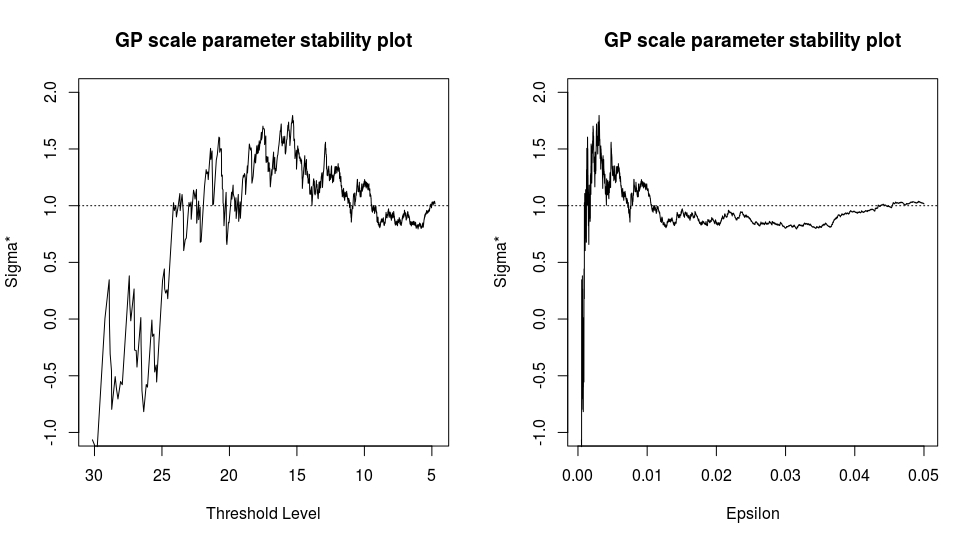
\includegraphics[width=\textwidth]{Figures/ThresholdVsEpsilon}
        \label{fig:comparison}
        \caption{Parameter estimates plotted against threshold levels on the left and tail quantiles on the right.}
    \end{figure}

The estimates for $\sigma^{*}$ used to plot both graphs in Figure \ref{fig:comparison} are exactly the same, yet one could draw opposite conclusions relating to stability when presented with both. It is clear that visually assessing stability is not feasible when the majority of estimate points are shifted to the right.

As our estimates are also independent of $\epsilon$ we can thus assess stability by fitting both distributions at a range of thresholds and then plotting all four estimates along with their confidence intervals against $\epsilon$. We can then select $\ell_0$ as the corresponding threshold level for the largest $\epsilon$ for which the four estimates remain constant up to minor sampling errors.

The confidence intervals for $\hat\alpha$, $\hat\xi$ and $\hat\sigma^{*}$ can be found in \cite{Cahoy2013}, \cite{Zhang2007} and \cite{ColesBook} respectively. A derivation of the confidence interval for $\hat\delta^{*}$ is provided in the appendix.

\section{Model Fit of Simulated Data}
In order to verify that our model is correct we will simulate bursty data such that we can theoretically calculate the true parameters of the ML and GP distributions. We will then apply our estimation method and compare our estimated parameters with the true parameters.

We wish to generate inter-arrival waiting times $W_k$ with the Laplace transform

$$\mathcal L_W(\lambda) = \E [e^{-\lambda W}] = e^{-\lambda^\alpha}$$ 
where $\alpha \in (0,1)$. 
The package R stabledist with option pm=1 runs with the parametrisation
as in Samorodnitsky \& Taqqu: (see Definition \ref{def:stableChar} for the full definition)
\begin{align*}
\phi_X (\theta) = \E[ e^{i\theta X}] = \exp \left\lbrace -\sigma^\alpha |\theta|^\alpha \left(1 - i\beta({\rm sign} \theta) \tan \frac{\alpha \pi}{2}\right) + i \mu \theta \right\rbrace.
\end{align*}
Hence we aim to find $\alpha, \beta, \sigma, \mu$ such that 
$$\mathcal L_W(-i\theta) = \phi_X(\theta), \quad \theta > 0.$$
Now see that 
\begin{align*}
e^{-(-i\theta)^\alpha}
&= \exp\left(-(\theta e^{-i \pi / 2})^\alpha\right)\\
&= \exp\left(-\left(\theta^\alpha e^{-i\alpha \pi/2}\right)\right)\\
&= \exp\left(-\theta^\alpha\left(\cos \frac{\alpha\pi}{2} - i \sin\frac{\alpha\pi}{2}\right)\right)
\\
&= \exp\left(-\theta^\alpha \cos\frac{\alpha\pi}{2}\left(1 - i \tan \frac{\alpha\pi}{2}\right)\right)\\
&=  \phi_X(\theta), \quad \theta > 0
\end{align*}
whenever $\sigma^\alpha = \cos\frac{\alpha\pi}{2}, \beta = 1, \mu = 0$. Thus we generate $W\sim S(\alpha,1,(\cos\frac{\alpha\pi}{2})^{1/\alpha},0)$ in order to get unit stable random variables. From \ref{eq:asymptoticPareto} we know that any stable law with stability parameter $\alpha$ has tails that are asymptotically equivalent to Pareto tails also with parameter $\alpha$. Thus $W\in RV(-\alpha)$, which implies that both the limit theorems (\ref{eq:partialSumLimit}) and (\ref{eq:renewalLimit}) hold. Moreover, recall from (\ref{eq:unitStable}) that we can pick $b(n)$ such that the stable subordinator $D(t)$ has Laplace transform $\E[e^{-\lambda D(t)}] = e^{-t \lambda^\alpha}$. Now in order for that to hold we need 
\[
	\frac{W_1 + \ldots + W_n}{b(n)} \overset{d}{\longrightarrow} D, \quad n \to \infty,
\]
where $D$ has Laplace transform $\E[e^{-\lambda D}] = e^{- \lambda^\alpha}$. Thus we need the following equality of Laplace transforms
\begin{align*}
	\E\left[\exp\left(-\lambda\left(\frac{W_1+\ldots+W_n}{b(n)}\right)\right)\right]&=\E\left[\exp\left(-\left(\frac{\lambda}{b(n)}W\right)\right)\right]^n\\
	&=\exp\left(-\left(\frac{\lambda}{b(n)}\right)^\alpha\right)^n\\
	&=\exp\left(-\lambda^\alpha\frac{n}{b(n)^\alpha}\right)\\
	&=e^{- \lambda^\alpha}
\end{align*}
whenever $b(n)=n^{1/\alpha}\in RV(1/\alpha)$ as expected.

For the event magnitudes we simply generate $J_k\sim GEV(\xi,\sigma,\mu)$ so that we can easily calculate the GP parameters of the exceedances. The sequence of i.i.d $\mathbb{R}^+\times\mathbb{R}$ random vectors $(W_k,J_k)$ then defines a heavy tailed renewal process, at whose renewal times GEV event magnitudes occurs as in Figure \ref{fig:bursty}.
	
	\begin{figure}[h]
        \centering
        \caption{Simulated bursty data}\label{fig:bursty}
% GENERAL REMARK: It's more accurate to call this process a max-renewal
% process (with heavy-tailed waiting times). Bursty process could also be a
% Hawkes process. You might want to update the title as well... happy to discuss.
        %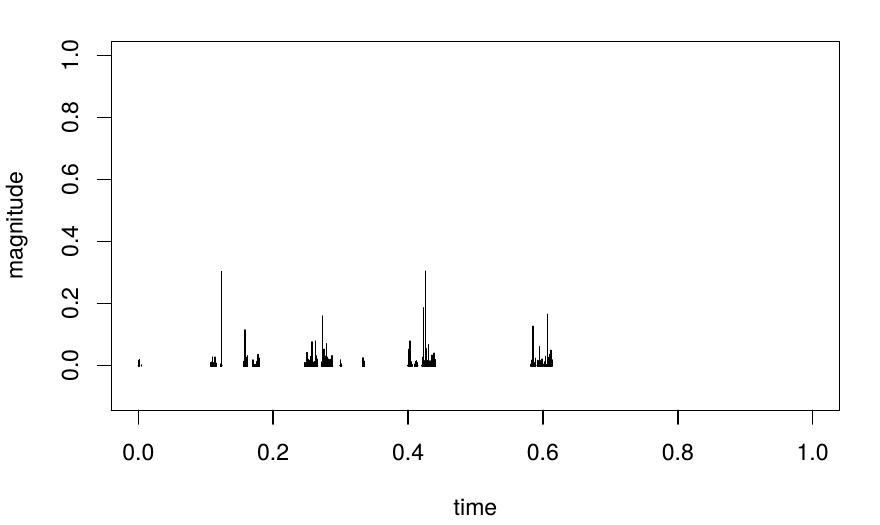
\includegraphics[width=\textwidth]{Figures/unitCTRMprocessNoTitle.png}
        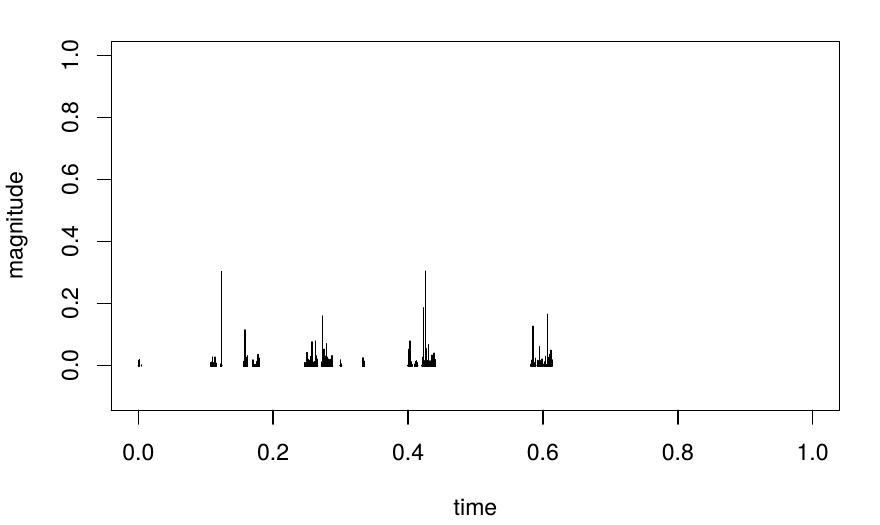
\includegraphics[width=\textwidth]{Figures/unitCTRMprocessNoTitle.png}
        %\label{fig:my_label}
    \end{figure}

Recall that we have defined the exceedance duration of level $\ell \in [x_0,x_F]$ as
the random variable
\begin{align*}
T_\ell = \inf\{t: V(t) > \ell\}
\end{align*}
and the exceedance as 
\begin{align*}
X_\ell = V(T_\ell) - \ell.
\end{align*}

Consider a minimum threshold $\ell_0$, e.g. at the 95\% quantile.
Vary the threshold $\ell$ on the interval $[\ell_0, x_F]$, and consider
the resulting sequences of exceedances and exceedance durations 
$\{(X_{\ell,i}, T_{\ell,i})\}$ as in Figure \ref{fig:thresholdedBursty}. 
Due to the renewal property every random variable in each sequence is i.i.d.. Thus $T_{\ell,1}, T_{\ell,2}, \ldots$ forms a simulated sample of exceedance durations and $J_{\ell,1}, J_{\ell,2}, \ldots$ forms a simulated sample of exceedances.


\begin{figure}[h]
    \centering
    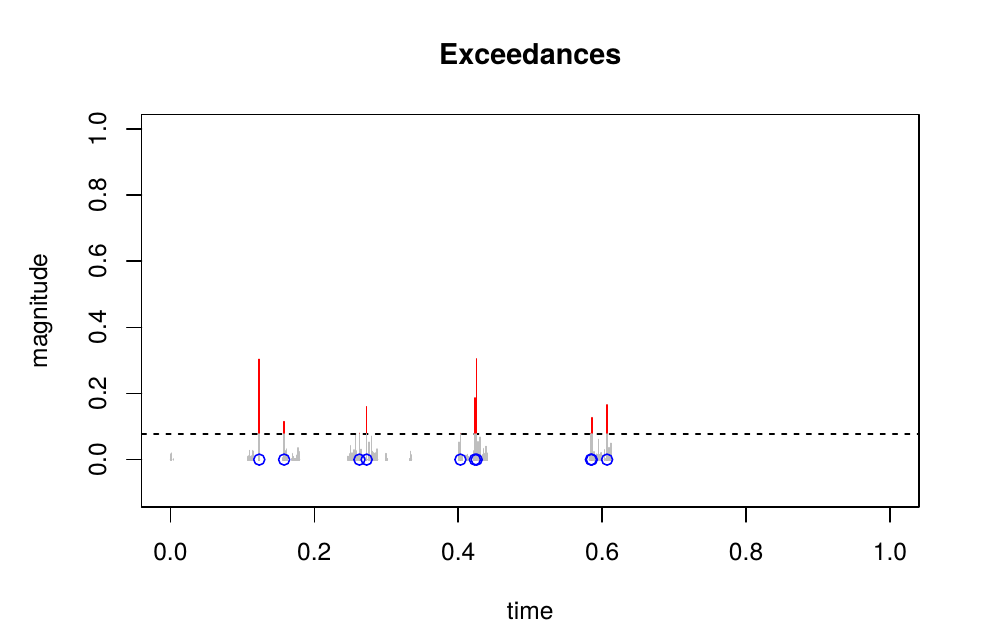
\includegraphics[width=\textwidth]{Figures/Exceedances.png}
    \caption{Exceedance durations (blue circles) and Exceedances (red lines).}\label{fig:thresholdedBursty}
    %\label{fig:my_label}
\end{figure}

We can now use the ML log moment estimator on the sample of exceedance durations and the GP likelihood moment estimator on the sample of exceedances to estimate all four parameters. Once we have parameter estimates for all thresholds $\ell$ on the interval $[\ell_0, x_F]$, we can graph our stability plots of $\hat \alpha$, $\hat\xi,$ $\hat\sigma^{*}$, and $\hat\delta^{*}$. Since we simulated data such that we could theoretically calculate the values of the adjusted parameters we know that $\delta^{*}=n^{1/\alpha}$ from (\ref{eq:deltaStar}) and $\sigma^{*}=\sigma-\xi\mu$ from (\ref{eq:sigmaStar}). 

%\begin{figure}[h]
%    \centering
%    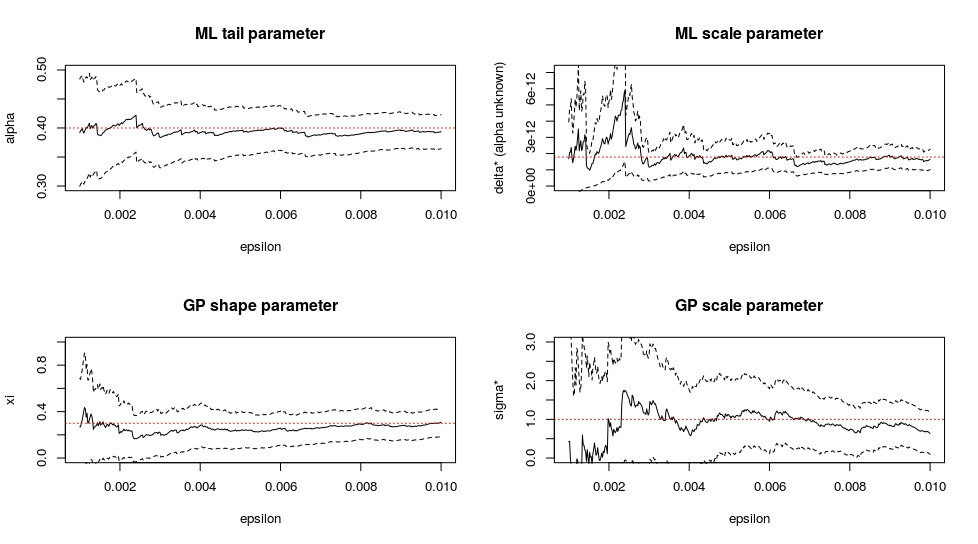
\includegraphics[width=\textwidth]{Figures/alphaUnknownFixed}
%    \caption{Exceedance durations (blue circles) and Exceedances (red lines).}\label{fig:thresholdedBursty}
%    %\label{fig:my_label}
%\end{figure}


\begin{figure}[h]
    \centering
    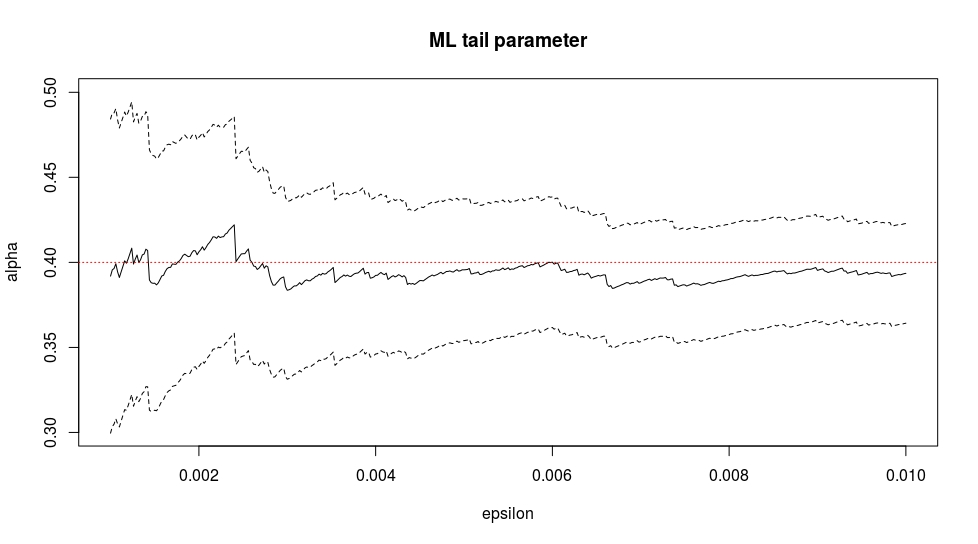
\includegraphics[width=\textwidth]{Figures/MLtail01}
    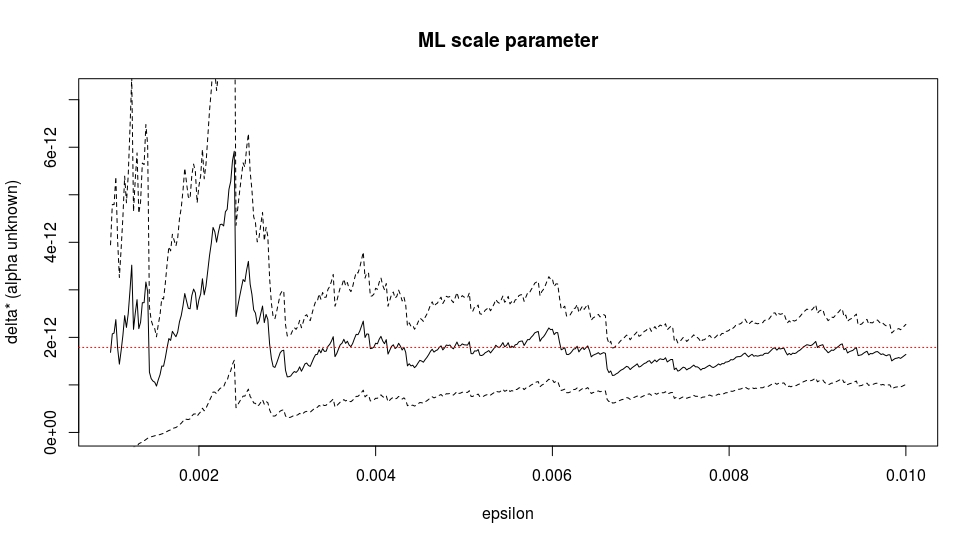
\includegraphics[width=\textwidth]{Figures/MLscale01}
    \caption{Mittag Leffler Stability Plots ($\alpha=0.4$, $n=50,000$)}\label{fig:MLstability}
    %n=50,000
\end{figure}

\begin{figure}[h]
    \centering
    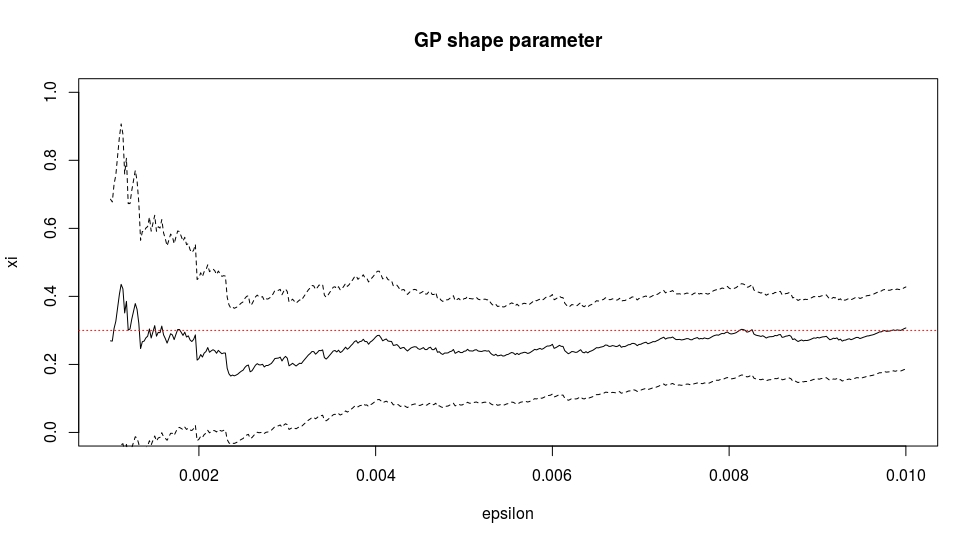
\includegraphics[width=\textwidth]{Figures/GPshape01}
    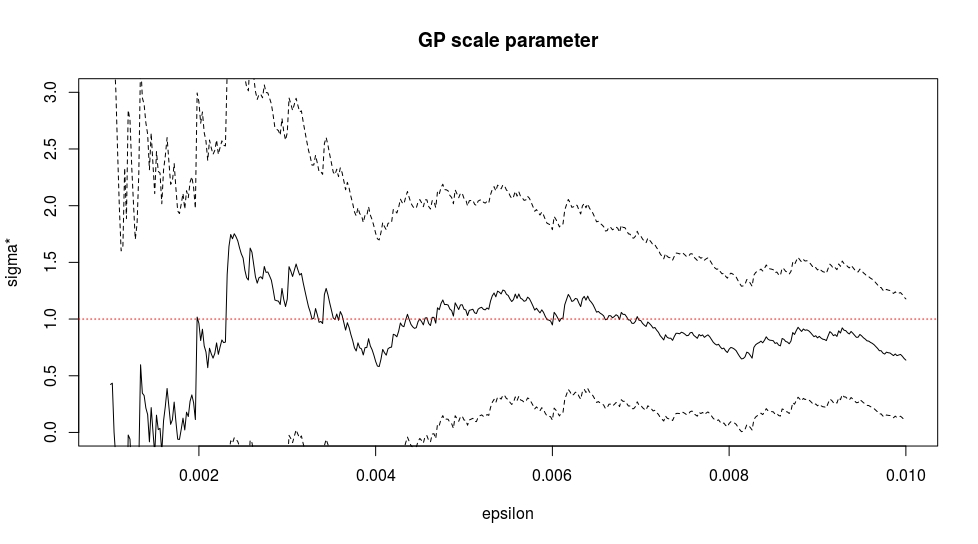
\includegraphics[width=\textwidth]{Figures/GPscale01}
    \caption{Generalised Pareto Stability Plots ($\xi=0.3$, $\sigma=1$)}\label{fig:MLstability}
\end{figure}
Both sets of plots look rather stable for the entire length of the plot, so using our threshold selection method we set $\ell$ as the threshold associated with $\epsilon=0.01$. This results in the following estimates
\begin{align*}
\hat \alpha &= 0.3935573\\
\hat \delta &= 1.957352\times10^{-7}\\
\hat \xi &= 0.3\\
\hat {\tilde \sigma} &= 3.682074.
\end{align*} 
Where the true values are \textcolor{red}{SOMETHING WRONG WITH b(n) HERE}
\begin{align*}
 \alpha &= 0.4\\
 \delta &= !!!??? \\
 \xi &= 0.3\\
 {\tilde \sigma} &= 1+\xi\ell =1+0.3\times 10.14632 = 4.043896
\end{align*} 
\chapter{Conclusion}


\chapter{Appendix}
From \cite{Cahoy2013} we know that
\[
\delta=\exp(\mu +\gamma)
\]
and
\[
\alpha=\sqrt{\frac{2\pi^2}{6\sigma^2+\pi^2}},
\]
where $\mu$ and $\sigma^2$ is the mean and variance of a log transformed Mittag-Leffler random variable. $\gamma=0.57721566490...$ is Euler's constant. We know that our space scaling constant can be defined in terms of the Mittag-Leffler parameters, that is
\[ 
b:=b(n)=\delta(-\log(F(\ell)))^{1/\alpha}.
\]
So we let $H(\delta,\alpha)=\delta(-\log(F(\ell)))^{1/\alpha}$ and then apply an appropriate Delta method to get a confidence interval for $b$. In 1996 Ferguson was able to show that \cite{Ferguson1996}
\begin{align*}
	\sqrt{n}\begin{pmatrix}
				\hat{\mu}-\mu\\
				\hat{\sigma^2}-\sigma^2\\				
			\end{pmatrix}
			\cd
			N\left(\begin{pmatrix}0\\0\\ \end{pmatrix},\Sigma	\right)
\end{align*}
where
\begin{align*}
	\Sigma=\begin{bmatrix}
		\sigma^2	& \mu_3\\
		\mu_3		& \mu_4-\sigma^4
	\end{bmatrix}.
\end{align*}
Note that $\mu_3$ and $\mu_4$ are the third and fourth central moments of the log transformed Mittag-Leffler random variable. Cahoy showed in \cite{Cahoy2013} that
\[
\mu_3=-2\zeta(3),
\]
where $\zeta(3)$ is the Riemann zeta function evaluated at 3, and
\[
\mu_4=\frac{\pi^4(\alpha^4-20\alpha^2+28)}{60\alpha^4}.
\] 
An application of the multivariate delta method gives
\begin{align*}
\sqrt{n}(\hat{b}-b)\cd N(0,\sigma^2_b)
\end{align*}
where
\begin{align*}
\sigma^2_b=(\nabla H)^T \Sigma (\nabla H)
\end{align*}
with
\begin{align*}
	\nabla H &=\begin{pmatrix}
		\ppartial{H}{\mu}\\
		\ppartial{H}{\sigma^2}\\
	\end{pmatrix}
	=\begin{pmatrix}
		\ppartial{H}{\delta}\times\ppartial{\delta}{\mu}\\
		\ppartial{H}{\alpha}\times\ppartial{\alpha}{\sigma^2}\\
	\end{pmatrix}.
\end{align*}
Now our partial derivatives are
\begin{align*}
\ppartial{H}{\delta}&=(-\log(F(\ell)))^{1/\alpha},\\ 
\ppartial{\delta}{\mu}&=\delta,\\
 \ppartial{H}{\alpha}&=-\frac{\delta}{\alpha^2}\log(-\log(F(\ell)))(-\log(F(\ell)))^{1/\alpha},\\ 
 \ppartial{\alpha}{\sigma^2}&=\frac{-3\sqrt{2}\pi}{(6\sigma^2+\pi^2)^{3/2}},
\end{align*}
so
\begin{align*}
	\nabla H &=\begin{pmatrix}
		b\\
		\dfrac{3\sqrt{2}\pi b \log(-\log(F(\ell)))}{\alpha^2(6\sigma^2+\pi^2)^{3/2}} \\
	\end{pmatrix},
\end{align*}
and it follows that
\begin{align*}
 \sigma^2_b= b^2\sigma^2 +\frac{b^2}{\alpha^2}\log(-\log(F(\ell)))
 \left[
 \frac{-12\sqrt{2}\pi\zeta(3)}{(6\sigma^2+\pi^2)^{3/2}} + \log(-\log(F(\ell)))\frac{32-20\alpha^2-\alpha^4}{40}
 \right].
\end{align*}
We have therefore shown that the log-moment estimate of $b$ is normally distributed for large $n$. Thus we can approximate the $(1-\epsilon)100\%$ confidence interval of $b$ as
\[
	\hat{b}\pm z_{\epsilon/2}\sqrt{\sigma^2_b}.
\]

%%%%%%%%%%%%%%%%%%%%%%%%%%%%%%%%%%%%%%%%%%%%%%%%%%%%%%%%%%%%%%%%%%%%%%%%%%

\clearpage
\addcontentsline{toc}{chapter}{References}
\bibliographystyle{alpha}
\bibliography{ThesisV1}

\end{document}
